% !TeX root = ../thuthesis-example.tex

\chapter{基于速率函数的随机块模型精确恢复问题研究}\label{chap:sibm}
\section{本章引言}
本章将利用速率函数这一信息论的度量研究
具有多个社团结构的随机块模型。具体来说,
我们的研究对象是
定义 \ref{def:SSBM} 中的 $\SSBM(n,k,\A, \B)$。
我们在之前的讨论中指出,当$\sqrt{a}-\sqrt{b}>\sqrt{k}$,即式 \eqref{eq:abk} 成立
时,存在实现精确恢复的算法,但实际问题中我们得到的是
随机块模型的实例,并没有$a,b$参数的信息,因此
我们在本章首先研究如何估计模型的参数 $a,b$。
此外,对于其他更高效的恢复算法,实现精确恢复的算法不一定由 式\eqref{eq:abk}
给出。
本章将研究一个具有辅助双参数$\beta,\gamma$ 的社团发现算法,
我们称之为基于玻茨模型的社团发现算法,
在研究这一算法的过程中,我们将展示如何利用速率函数刻画其精确恢复条件
和误差衰减率等性质。进一步地,我们将研究由玻茨模型
衍生出的社团发现算法的误差率,
该方法为基于能量最小化的社团发现算法。
上述算法便于理论分析但实际实现只能近似求解。
为此,我们采用梅特罗波利斯采样算法进行近似,
通过该近似算法的实验结果我们将验证$\beta$参数对误差率的影响。

本章内容的具体安排如下:
在 \ref{sec:parameter_estimation} 节,我们首先研究了
随机块模型的超参估计问题;
在 \ref{sec:potts} 节,我们研究了基于玻茨模型的社团发现算法
的相变现象和恢复误差;接下来,
在 \ref{sec:em} 节,我们分析了基于能量最小化的社团发现算法
的恢复误差;在 \ref{sec:ms} 节,用梅特罗波利斯采样对
玻茨模型的相变现象进行了验证;第 \ref{sec:sibm_proof} 节给出了本节提出的
定理的证明;
第 \ref{sec:summary_potts} 节对全章进行了总结。
\section{参数估计}\label{sec:parameter_estimation}


本节中,我们考虑 $\SSBM(n,k,\A, \B)$ 模型的参数估计
问题。关于 随机块模型 的参数估计问题也有相关的研究工作。
在几乎一致恢复的场景下 Mossel 提出了参数 $(a,b)$ 的一个一致估计量
\cite{mossel2015reconstruction}。
而对于精确恢复的情形,通常可以先恢复节点的标签,再估计模型参数
\cite{abbe2015recovering}。

假设 $k$ 已知,
我们想从图 $G$ 中估计
$a$ 和 $b$。
我们提出的方法如下,首先
对$G$中 边的数量 $T_1$ 
和 三角形的数量
$T_2$进行计数,然后通过求解下述
关于$(x,y)$的非线性方程组得到
估计量 $\hat{a}, \hat{b}$:
\begin{equation} \label{eq:e_1}
\left\{
	\begin{alignedat}{1}
	\frac{x+(k-1)y}{2k}  &= \frac{T_1}{n\log n} \\
\frac{1}{k^2}
\left(\frac{x^3}{6} + \frac{k-1}{2}xy^2 + (k-1)(k-2)\frac{y^3}{6}\right)
 &= \frac{T_2}{\log^3 n}
	\end{alignedat}
\right.
\end{equation}


解的理论保证由如下定理给出:
\begin{theorem}\label{thm:ab12}
当 $n$ 足够大时,
关于方程组\eqref{eq:e_1}
有唯一解 $x=\hat{a}, y=\hat{b}$,
\newglossaryentry{consistent_est}{name=一致估计量, description={Consistent estimator}}
并且该解是参数$(a,b)$的\gls{consistent_est},
也即 $\hat{a}, \hat{b}$ 
分别依概率收敛到 $a,b$ 。
\end{theorem}
给定一个由随机块模型生成的图,
我们可以用定理 \ref{thm:ab12} 获得参数$a,b$ 
的估计量,然后用 \eqref{eq:abk}
式
来判断标签$X$ 的精确恢复是否可能。
此外,对于有限规模的图,定理 \ref{thm:ab12} 提供的 $a,b$ 的估计可用于
初始化某些恢复算法的相关参数,
比如最大似然估计或者我们
将在 \ref{sec:ms} 节使用的梅特罗波利斯算法。

下面我们通过实验来验证
定理 \ref{thm:ab12} 的结果。我们考虑若干组不同的
$(a,b,k)$ 的组合,对于每一种取值,
通过定理 \ref{thm:ab12} 我们可得到估计量
\newacronym{acr:mse}{MSE}{Mean square error}
$(\hat{a}, \hat{b})$,进而计算
均方误差(\gls{acr:mse})
$\frac{1}{m} \sum_{i=1}^m (\hat{a}-a)^2 + (\hat{b}-b)^2$。
这里  采样次数$m$ 取 $1000$。
实验结果 如
图 \ref{fig:estimator} 所示。
由此可见, 随着 $n$ 的增大,
均方误差 以多项式的速率减小。
从而验证了 $\hat{a}, \hat{b}$ 分别收敛到 $a,b$ 
的结果。

\begin{figure}[ht!]
	\centering
		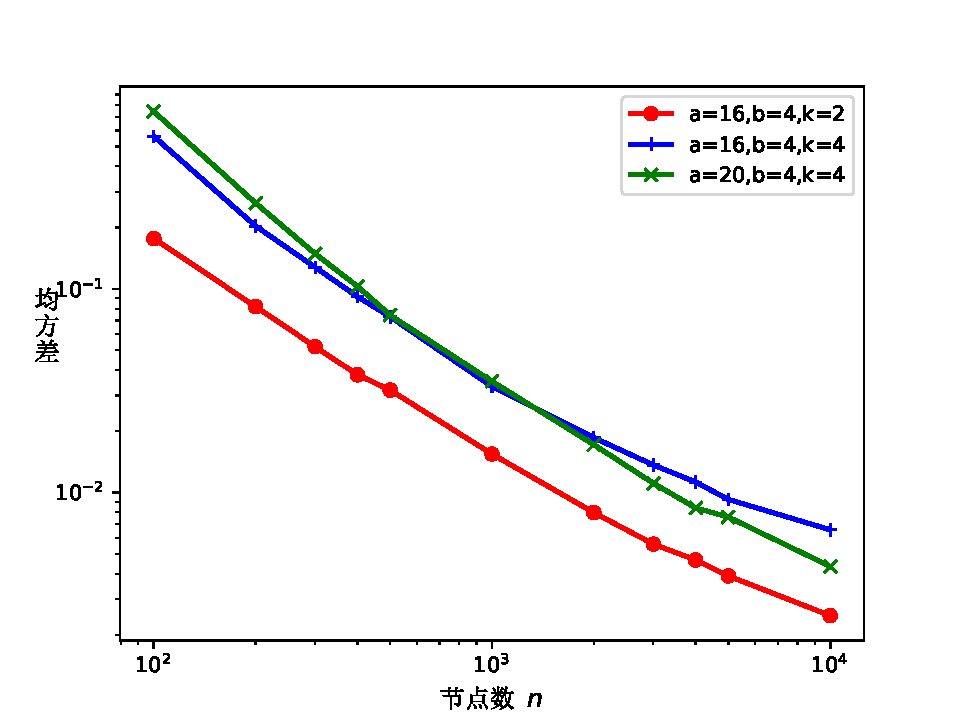
\includegraphics[width=0.6\textwidth]{estimator-error-2023-03-10.pdf}
		\caption{ $\hat{a}, \hat{b}$ 的估计误差随
		$n$ 的变化规律 }\label{fig:estimator}
\end{figure}

\section{基于玻茨模型的社团发现算法}\label{sec:potts}
\subsection{算法描述}
类似于 \ref{sec:ising} 节
介绍的SIBM模型,我们将
随机块模型
与 \ref{sec:ising} 节介绍的 玻茨模型
复合起来可得到随机块-玻茨模型。该模型可以看成是SIBM模型的推广,
每个节点由两状态变成了多状态。我们的研究重点是
从随机块-玻茨模型生成的一个样本$\sigma$恢复节点的原始标签$X$,相当于利用
玻茨模型对随机块模型进行社团发现。为此,我们首先给出
在随机块模型生成的图上定义的玻茨模型:
\begin{definition}\label{def:ising}
	给定从$\SSBM(n,k,\A,\B)$ 中生成的随机图 $G$,
    定义在$G$上的玻茨模型($k$个状态的伊辛模型)是关于状态向量$\sigma\in W^n$ 的概率分布
。该分布有两个参数 $\beta, \gamma>0$,其概率质量函数为
\begin{align} \label{eq:isingma}
	P_{\sigma|G}(\sigma=\bar{\sigma})=\frac{\exp(-\beta H(\bar{\sigma}))}{Z_G(\beta, \gamma)}
	\end{align}
其中能量函数$H(\bar{\sigma})$的定义是
\begin{equation}\label{eq:energy}
	H(\bar{\sigma}) := \gamma \frac{\log n}{n} \sum_{(i,j)\not\in E(G)} \delta(\bar{\sigma}_i, \bar{\sigma}_j)
	- \sum_{(i,j)\in E(G)} \delta(\bar{\sigma}_i, \bar{\sigma}_j)
	\end{equation}
	
	$P_{\sigma|G}$ 中的下标表示节点状态$\sigma$的分布依赖于$G$,
    $Z_G(\beta, \gamma)$ 是该分布的归一化常数。
\end{definition}

式\eqref{eq:isingma}中
各符号的含义同式\eqref{eq:canonical_ensemble}。
而表示汉密尔顿能量的式\eqref{eq:energy}
则是式\eqref{eq:ising_modified}的推广。
当  $k=2$ 时,式 \eqref{eq:energy}
在注释 \ref{rem:equivalence_H_energy} 的意义下
退化成 式 \eqref{eq:ising_modified}。 

这里的能量函数$H(\bar{\sigma})$ 同样有两部分组成:
没有边相连的节点之间排斥力的势能和
有边相连的节点之间吸引力的势能。
$\gamma$ 是没有边相连的节点间的作用力系数。
考虑到两节点间有边相连的概率仅为 $O\left(\frac{\log n}{n} \right)$,
$\frac{\log n}{n}$ 是对由于边的数量不均匀造成两种势能量阶不同的修正项。


定义\ref{def:ising}说明了 $X \leftrightarrow G \leftrightarrow \sigma$构成了马尔可夫链。
由此我们得到一个$X$的估计量 $\hat{X}^*=\sigma$。
这里,估计量 $\hat{X}^*$ 表示由玻茨模型生成的一个样本,
记作$\hat{X}^* \sim \textrm{Potts}_G(\beta, \gamma)$。
下面我们首先研究$\hat{X}^*$实现精确恢复的条件及误差上界,
而关于如何进行玻茨模型的采样我们将在后面进行讨论。
\subsection{误差的渐近性质}
沿用注释 \ref{rem:metric_exact_recovery} 中的记号,
使用$\hat{X}^*$估计$X$在精确恢复度量下的错误概率
记为 $P_e(\hat{X}^*) := \sum_{\bar{G} \in \cG_n}
P_G(\bar{G}) P_{\sigma | \bar{G}}(\hat{X}^* \in S^c_k(X))$。
类似文献 \inlinecite{ye2020exact} 中关于 SIBM 模型的讨论,
玻茨模型的两个参数$(\beta, \gamma)$ 的取值
对$P_e(\hat{X}^*)$
也有着决定性的作用。
当它们取合适的值时, 
$ P_e(\hat{X}^*)\to 0$,
随机块模型的精确恢复可以实现。
反之,如果 $(\beta, \gamma)$ 取其他值时,
$P_e(\hat{X}^*) \to 1$,即$P_a(\hat{X}^*) \to 0$。
这两种情况可总结为如下的定理:

\begin{theorem}\label{thm:phase_transition}
	假设 $\sqrt{a} - \sqrt{b} > \sqrt{k}$,
	定义函数 $g(\beta)$ 和 $ \tilde{g}(\beta)$ 如下:
	\begin{equation}
		\label{eq:g_beta_main_article}
		g(\beta) = \frac{be^{\beta} + a e^{-\beta}}{k} - \frac{a+b}{k} +1
	\end{equation}
	且
	\begin{equation}
		\label{eq:g_tilde_beta_main_article}
	\tilde{g}(\beta) = \begin{cases}
	g(\beta) & \beta \leq \bar{\beta} = \frac{1}{2}\log \frac{a}{b} \\
	g(\bar{\beta}) = 1 - \frac{\left(\sqrt{a} - \sqrt{b}\right)^2}{k} & \beta > \bar{\beta}
	\end{cases}
	\end{equation}
	其中
	$\bar{\beta} =  \displaystyle\argmin_{\beta > 0} g(\beta)$。
	令 $\beta^*$ 定义成
	\begin{equation}\label{eq:beta_star}
	\beta^* = \log\left(\frac{a + b - k - \sqrt{(a + b - k)^2 - 4 a b}}{2  b}\right)
	\end{equation}
	可以验证 $\beta^*$ 是方程 $g(\beta) = 0$ 的解 并且满足  $\beta^* < \bar{\beta}$。	
	设 $G\sim \SSBM(n, k, \A, \B)$, $\hat{X}^* \sim \textrm{Potts}_G(\beta, \gamma)$,
	对于给定的 $\epsilon > 0$, 当 $n$ 充分大时, 我们有:
	\newglossaryentry{not:small_o}
	{
	  type=notation,
	  name={$o(1)$},
	  description={无穷小量}
	}
	\begin{enumerate}
	\item 当 $\gamma > b$ 且 $\beta > \beta^*$ 时,$P_e(\hat{X}^*) \leq n^{\tilde{g}(\beta)/2 + \epsilon}$;
	\item 当 $\gamma > b$ 且 $\beta < \beta^*$ 时,$P_a(\hat{X}^*) \leq (1+$\gls{not:small_o}$)\max\{n^{g(\bar{\beta})}, n^{-g(\beta) + \epsilon}\}$;
	\item 当 $\gamma < b$ 时,对于任意给定的 $C>0$	均有 $P_a(\hat{X}^*) \leq \exp(-C n)$。
	\end{enumerate}
\end{theorem}

\begin{figure}[H]
	\begin{subfigure}{0.43\textwidth}
		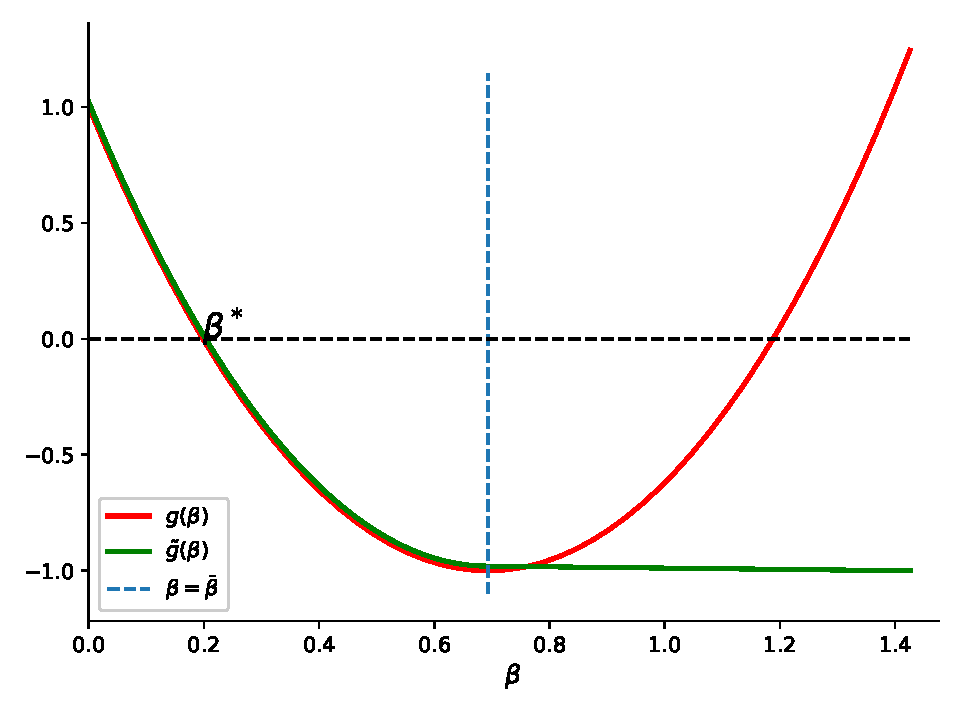
\includegraphics[width=\textwidth]{g-16-4-2.pdf}
		\caption{当 $a=16,b=4,k=2$时,$g(\beta)$和
		$\tilde{g}(\beta)$的函数图像}\label{fig:g}
	\end{subfigure}~
	\begin{subfigure}{0.55\textwidth}
		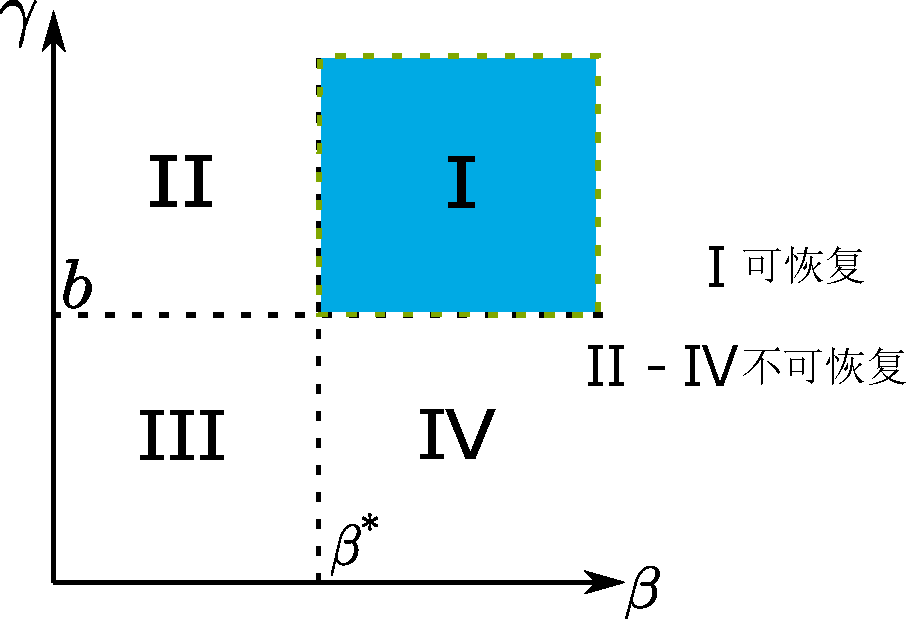
\includegraphics[width=\textwidth]{phase_trans_chinese.pdf}
		\caption{
			在 $(\beta, \gamma)$ 平面内
			相变区域图示。
			随机块模型的精确
			恢复仅在区域 I 可实现。}\label{fig:pt}
	\end{subfigure}
	\caption{定理 \ref{thm:phase_transition} 
	的图示}
	\label{fig:phase_transition_theorem_illustration}
\end{figure}
\begin{remark}
	在式\eqref{eq:g_beta_main_article} 中,我们首次引入了
	$g(\beta)$ 这个函数,该函数是由矩生成函数导出的,
	其信息学含义为速率函数的凸共轭函数,
	具体我们将在 \ref{sub:rate_function} 小节专门讨论。
\end{remark}
%与式\eqref{eq:beta_star_sibm}的情形类似,
注意到条件$\sqrt{a} - \sqrt{b} > \sqrt{k}$使得
式\eqref{eq:beta_star}中根号下的项非负。
这个条件来自于定理 \ref{thm:sbmk_phase_transition},
保证了随机块模型本身精确恢复可实现。


通过简单的计算可知,对于 $\beta> \beta^*$,
我们有 $\tilde{g}(\beta) < 0$,
而 对于 $\beta < \beta^*$,有
$g(\beta)>0$。
另外,由 $\sqrt{a} - \sqrt{b} > \sqrt{k}$ 可知
$g(\bar{\beta}) < 0$。
$g(\beta), \tilde{g}(\beta)$ 的图像
如图 \ref{fig:phase_transition_theorem_illustration} (a)所示。
因此, 对于充分小的
$\epsilon$ 并且当 $n \to \infty$,
定理 \ref{thm:phase_transition} 中给出的上界
均至少以多项式的速度趋向于 $0$。
从而定理 \ref{thm:phase_transition} 刻划了
玻茨模型的相变性质。
如图 \ref{fig:phase_transition_theorem_illustration} (b)所示
, 对于玻茨模型, 只有参数$(\beta, \gamma)$落在区域I时,
随机块模型的精确
恢复才能实现。



定理 \ref{thm:phase_transition} 中的$k=2$与
文献\inlinecite{ye2020exact}的定理2中的$m=1$时
的结论是一致的。此外,
定理 \ref{thm:phase_transition} 也
可以从$\sigma$的边缘分布的角度理解。
玻茨模型取到某个特定状态$\bar{\sigma}$的概率为
 $P_{\sigma}(\sigma =\bar{\sigma})
=\sum_{\bar{G} \in \cG_n}P_G(\bar{G})
P_{\sigma |\bar{G}}(\sigma=\bar{\sigma})$。
下面考虑$\sigma$离$X$较近时$\sigma=X$的概率。
为此,定义函数
\begin{equation}
	\label{eq:D_sigma_sigma_prime}
\Phi(\sigma, \sigma') := \mathds{1} [ \Dist(\sigma, \sigma')  = \min_{f \in S_k} \Dist(f(\sigma), \sigma')  \}]
\end{equation}
则  $\Phi(\sigma, \sigma')=1$ 时, $\sigma$ 相比于它的所有置换其本身离 $\sigma'$ 最近。

由定理 \ref{thm:phase_transition}, 对边缘分布 $P_{\sigma}$ 我们有如下论断
:
\begin{corollary}\label{cor:phase4}
假设 $\gamma > b$, $X$满足定义 \ref{def:SSBM} 中的约束,取决于 $\beta$ 的取值我们有
\begin{enumerate}
	\item 当 $\beta > \beta^*$时,$P_{\sigma}(\sigma = X | \Phi(\sigma, X)=1)  = 1-o(1)$;
	\item 当 $\beta < \beta^*$时,$P_{\sigma}(\sigma = X | \Phi(\sigma, X)=1)  = o(1)$。
\end{enumerate}
\end{corollary}

下面我们简单阐述下 定理 \ref{thm:phase_transition} 证明的思路。
该思路主要通过对翻转一个状态的前后能量差的分析来估计概率的主项。
下面的引理总结了翻转一个状态前后汉密尔顿能量的变化:
\begin{lemma}\label{lem:lemmaDiff}
	假设 $\bar{\sigma}'$ 仅在第$r$个位置上与 $\bar{\sigma}$ 不同,
	差别为 $\bar{\sigma}'_r = \omega^s \cdot \bar{\sigma}_r$。
	则 $\bar{\sigma}'$ 和 $\bar{\sigma}$ 的能量差为
\begin{align}
	H(\bar{\sigma}') - H(\bar{\sigma}) &= \left(1+\gamma \frac{\log n}{n} \right)
	\sum_{i \in N_r(G)} J_s(\bar{\sigma}_r, \bar{\sigma}_i)
	+ \gamma \frac{\log n}{n} (m(\omega^s \cdot \bar{\sigma}_r)-m(\bar{\sigma}_r)+1) \label{eq:DeltaH}
	\end{align}
	上式中 $m(\omega^j) := \left|\left\{i \in [n] | \bar{\sigma}_i = \omega^j \right\} \right| $,
	$N_r(G):=\{j | (r, j) \in E(G) \}$ 表示节点$r$
	的邻居节点,
	而 $J_s(x, y) = \delta(x, y) - \delta(\omega_s \cdot x, y)$。
\end{lemma}
\begin{proof}
	首先我们将
  \eqref{eq:energy} 式改写成
	\begin{equation*}
	H(\bar{\sigma}) = \gamma \frac{\log n}{n} \sum_{i < j} \delta(\bar{\sigma}_i, \bar{\sigma}_j)
	- \left(1 + \gamma\frac{\log n}{n} \right)
	\sum_{ (i,j) \in E(G)} \delta(\bar{\sigma}_i, \bar{\sigma}_j)
	\end{equation*}
	
	接着我们逐步计算能量差:
  \begin{align*}
	H(\bar{\sigma}') - H(\bar{\sigma}) =& 
  \left(1 + \gamma\frac{\log n}{n}
  \right)
   \sum_{i \in N_r(G)} (\delta(\bar{\sigma}_r, \bar{\sigma}_i) -
	\delta(\omega^s \cdot \bar{\sigma}_r, \bar{\sigma}_i)) \\
	&+ \gamma \frac{\log n}{n}\sum_{i\neq r}
	( \delta(\omega^s \cdot \bar{\sigma}_r, \bar{\sigma}_i) -
	\delta( \bar{\sigma}_r, \bar{\sigma}_i) ) \\
	 =& \left(
     1 + \gamma\frac{\log n}{n}
     \right)
   \sum_{i \in N_r(G)} J_s(\bar{\sigma}_r, \bar{\sigma}_i) \\
	&+ \gamma \frac{\log n}{n}\sum_{i=1}^n
	( \delta(\omega^s \cdot \bar{\sigma}_r, \bar{\sigma}_i) -
	\delta( \bar{\sigma}_r, \bar{\sigma}_i) +1) \\
	=& \left(1+\gamma \frac{\log n}{n}
  \right)
  \sum_{i \in N_r(G)} J_s(\bar{\sigma}_r, \bar{\sigma}_i)\\
	&+ \gamma \frac{\log n}{n} (m(\omega^s \cdot \bar{\sigma}_r)-m(\bar{\sigma}_r)+1)
	\end{align*}
\end{proof}
\begin{remark}\label{re:energy_diff}
	当 $\bar{\sigma}'$ 与 $X$ 仅在位置 $r$
	上不同时, 在引理 \ref{lem:lemmaDiff} 中
	取$\bar{\sigma}=X$,
	结合条件  $|\{v \in [n] | X_v = u\}| = \frac{n}{k}$,
	有 $m(\omega^s \cdot \bar{\sigma}_r)
	=m(\bar{\sigma}_r)$,
	进而:
	\begin{equation}\label{eq:energy_diff}
	H(\bar{\sigma}') - H(X) = \left(1+\gamma \frac{\log n}{n} \right)
	(A^0_r - A^s_r) + \gamma\frac{\log n}{n}
	\end{equation}
	其中 $A^s_r$ 定义成
	$A^s_r := |\{j \in [n]\backslash \{r\} | \{j, r\} \in E(G), X_j = \omega^s \cdot X_r \}|$。
	因为$G$中各边的存在与否是独立的,
	对于 $s\neq 0$
	我们有 $A^s_r \sim \Binom \left(
	  \frac{n}{k}, \B \right) $,
	  即参数为$\frac{n}{k}, \B$的二项分布,
	而 $A^0_r \sim \Binom
	\left(
	  \frac{n}{k}-1, \A \right)$。	
\end{remark}
考虑到:
\begin{equation}\label{eq:Pratio}
\frac{P_{\sigma |G } (\sigma = \bar{\sigma}')}{P_{\sigma |G } (\sigma = \bar{\sigma})}
= \exp(-\beta(H(\bar{\sigma}') - H(\bar{\sigma})))
\end{equation}
因此引理 \ref{lem:lemmaDiff} 提供了用以比较两个相邻状态的概率
的方法。当 $n$充分大时,我们注意到式
\eqref{eq:Pratio} 右端化为$\exp(-\beta (A_r^0 - A_r^s))$。
而如果我们对其取期望,则可以得到
\begin{equation}\label{eq:expect_A_r_0_s}
	\E[\exp(-\beta (A_r^0 - A_r^s))] \sim n^{g(\beta)-1}
\end{equation}
也即 $g(\beta)$与两个二项分布差$A_r^0 - A_r^s$的矩生成函数有关。



另外, 我们注意到 因为图中边的数量是稀疏的,每个节点
平均有 $O(\log n)$ 个相连的邻居节点。
按照式 \eqref{eq:DeltaH} 
计算能量差的时间复杂度也是 $O(\log n)$。

当 $H(\bar{\sigma}') > H(\bar{\sigma})$ 时, 
由式\eqref{eq:Pratio} 可得
$P_{\sigma | G}(\sigma = \bar{\sigma}')<P_{\sigma | G}(\sigma = \bar{\sigma})$。
粗略而言, 如果
$ \sum_{\Dist(\bar{\sigma}', X)=1}\exp(-\beta(H(\bar{\sigma}') - H(X))) $
收敛到零,
我们可以预期,与$S_k(X)$不同的所有其他状态的概率收敛到零,
即$P_{\sigma}(S_k(X))$趋于1。
与之相反, 如果
$ \sum_{\Dist(\sigma', X)=1}\exp(-\beta(H(\bar{\sigma}') - H(X))) $
趋于无穷大,
则 $P_{\sigma}(S_k(X))$ 趋于零。
此种分析展示了证明定理 \ref{thm:phase_transition} 的
主要思路。应用这一思路,由式
\eqref{eq:expect_A_r_0_s},
当$n$充分大时,$ \sum_{\Dist(\bar{\sigma}', X)=1}\exp(-\beta(H(\bar{\sigma}') - H(X))) $
的数学期望为 $n^{g(\beta)}$,
通过讨论$g(\beta)$的正负可以部分说明
定理 \ref{thm:phase_transition} 中的表述。

\subsection{误差衰减率与速率函数}\label{sub:rate_function}
定理 \ref{thm:phase_transition} 除了给出定义在随机图上的
玻茨模型的相变现象外,
还给出了精确恢复条件下的误差衰减率。当$\beta^*<\beta<\bar{\beta}$时,
该速率为$n^{g(\beta)/2}$。
在\eqref{eq:expect_A_r_0_s} 中我们指出了$g(\beta)$与
二项分布差$A_r^0 - A_r^s$的矩生成函数有关,本节将进一步挖掘
其信息论的含义。

首先,通过切尔诺夫不等式的方法
(证明见附录引理 \ref{lem:enhanced_fb} ),
我们有
\begin{equation}\label{eq:introduction_g_a_b_eps}
  P_G(A_r^s - A_r^0 \ge t  \log n) 
	\le  \exp\left(-\log n \cdot
	\left(
   \frac{1}{k} g(a,b,kt) + O\left((\log n)^{-\delta} \right) \right)\right)
\end{equation}
其中 函数 $g(a,b,\epsilon)$ 的定义为
\begin{equation}  \label{equation:g}
  g(a,b,\epsilon) \triangleq a + b - \sqrt{\epsilon^2 + 4ab} + \epsilon \log \frac{\epsilon + \sqrt{\epsilon^2 + 4ab}}{2b}
\end{equation}
其等价形式亦可参见 文献\inlinecite{abbe2015exact} 中的 式 (43)
。
易验证
% $\frac{g(a,b,kt)}{k}=-[f_{\beta}(t)-\beta t -1]$。
%实际上
$g(a,b,s)$ 和 $g(s)-1$ 互为凸共轭函数(定义 \ref{def:convex_conjugate} )。

利用凸共轭函数的概念,
下面我们引入大偏差理论中的 Gärtner Ellis 定理
来获得 $g(a,b,\epsilon)$。Gärtner Ellis 定理是
Cramér 定理(定理 \ref{thm:cramer} )的推广,
其一般情形下的表述可参见
文献\inlinecite{dembo2009large}。
我们这里仅给出 Gärtner Ellis 定理的一个特例形式。

令 $S_n$ 为随机变量的序列,
$\gamma_n >0, \lim_{n\to \infty}\gamma_n \to \infty$。
$\Lambda_n(t)=\log \E[\exp(t S_n)]$ 代表 $S_n$ 的对数矩生成函数。
假设对于任意的 $t$,
$\Lambda(t) =\lim_{n\to \infty} \frac{1}{\gamma_n}\Lambda_n(\gamma_n t)$
存在。 令 $\Lambda^*$ 是 $\Lambda$ 的共轭函数。
则对于任意 紧集 $\Gamma \subset \mathbb{R}$,
我们有
\begin{equation}\label{eq:gartner_ellis}
\lim_{n\to \infty} \frac{1}{\gamma_n}\log P(S_n \in \Gamma) = -\inf_{s \in \Gamma} \Lambda^*(s)
\end{equation}
仿照 Cramér 定理中速率函数的概念,这里我们也把$\Lambda^*(s)$叫做速率函数。

下面我们应用式 \eqref{eq:gartner_ellis}
导出 $g(a,b,\epsilon)$ 的
表达式。
我们取 $\gamma_n= \log n$ 且 $\gamma_n S_n = \sum_{i=1}^n Y_i$,$Y_i=Z_i - W_i$,
$Z_i, \dots, Z_n$ 是 i.i.d. $\Bern\left(\B\right)$ 而 $W_1, \dots, W_n$ 是 i.i.d. $\Bern\left(\A\right)$。
$Y_i$ 的概率质量函数可表示为 $[(1-q)p, qp+(1-p)(1-q), q(1-p)]$,对应 $[-1,0,1]$ 三个取值。
首先我们计算得到 
$\Lambda(t) = \lim_{n\to \infty} \frac{n}{\log n} \log \E[\exp(t Y_1)]
=-a-b+be^t  + ae^{-t}$。
由 $\Lambda^*(s) = \sup_{t\in\mathbb{R}}\ st - \Lambda(t)$,
我们进一步得到 $\Lambda^*(s) = g(a,b,s)$。

在我们的问题中, $\Gamma=[t, +\infty)$ 。
考虑到 $\Lambda^*(s)$  是$[0,+\infty)$ 上的增函数,
我们有
\begin{equation}
  \lim_{n\to \infty} \frac{1}{\log n} P(S_n \ge t \log n)
  = g(a,b,t)
\end{equation}
该结果是式\eqref{eq:introduction_g_a_b_eps} 中 $k=1$结果的极限情况。
特别地,当$t=0$ 时, $g(a,b, 0) = \left(\sqrt{a} - \sqrt{b}\right)^2$。

\section{基于能量最小化的社团发现算法}\label{sec:em}
因为 $\beta^*$ 和 $n$ 无关,
当 $\gamma>b$ 时,
我们可以选取一个足够大的 $\beta$ 使得
$\beta > \beta^*$,
则 由 定理 \ref{thm:phase_transition},
当$n$充分大时 $\sigma \in S_k(X)$ 几乎必然发生。
这蕴含了 $P_{\sigma | G}(\sigma = X)$
对于几乎所有 从 随机块模型生成的图  $G$来说 取得最大值。
因此
相比于从玻茨模型中采样的方法,我们可以直接最大化条件概率,以
找到概率最大值的状态。
等价地, 我们可以通过最小化 式\eqref{eq:energy}来获得状态的估计量:
\begin{equation}\label{eq:hatX}
\hat{X}' := \argmin_{\bar{\sigma} \in W^n} H(\bar{\sigma})
\end{equation}

在 \eqref{eq:hatX} 中, 我们让 $\bar{\sigma}$ 在 $W^n$ 中取值。
因为我们已知 $X$取各个标签的位置数相等,即对于每个标签值 $u$
有 $|\{v \in [n] : X_v = u\}| = \frac{n}{k}$,
我们可以把搜索空间限制到
$W^*:= \left\{\sigma\in W^n \Big\vert |\{v \in [n] : \sigma_v = \omega^s\}| = \frac{n}{k}, s=0,\dots, k-1 \right\}$
上。
当 $\sigma \in W^*$ 时, 最小化 $H(\sigma)$ 等价于:
\begin{equation}\label{eq:hatX_double_prime}
\hat{X}'' := \argmin_{\sigma \in W^*} \sum_{(i,j) \not\in E(G) } \delta(\sigma_i, \sigma_j)
\end{equation}
其最小值是不同社团之间的最小分割。

当 $\hat{X}'' \neq X$ 时,
我们必须有  $\Dist(\hat{X}'' ,X)\geq 2$
以满足 硬约束 $\hat{X}'' \in W^*$。
此外,估计量 $\hat{X}''$ 是无参的,而 $\hat{X}'$的值受
参数 $\gamma$ 的影响。
在
$\hat{X}'$ 的表达式中出现的额外的参数 $\gamma$ 可视为
某种整数规划的拉格朗日乘子。
因此,通过引入惩罚因子项和将搜索空间从$W^*$ 扩大 到$W^n$
,求解 $\hat{X}''$
的优化问题 转变为求解 $\hat{X}'$的问题。

当 $\beta > \bar{\beta}$ 时,
$\tilde{g}(\beta)$ 是一个常数。
因此,从定理 \ref{thm:phase_transition} 中我们可以获得的关于
玻茨模型的估计量 $\hat{X}^*$ 最紧的上界
是  $n^{g(\bar{\beta})/2}$。

对于 $\hat{X}'$ 和 $\hat{X}''$ 这两个估计量,
我们可以获得 更紧的误差上界。我们把这一结果总结为如下定理:
\begin{theorem}\label{thm:error_rate}
当 $\sqrt{a} - \sqrt{b} > \sqrt{k}$ 时,
对于充分大的 $n$,我们有 
\begin{enumerate}
	\item 若 $\gamma > b$, $P_G(\hat{X}' \not\in S_k(X)) \leq (k-1+o(1))n^{g(\bar{\beta})}$;
	\item $P_G(\hat{X}'' \not\in S_k(X)) \leq \left((k-1)^2+o(1) \right)n^{2g(\bar{\beta})}$。
\end{enumerate}
\end{theorem}
因为 $g(\bar{\beta})<0$, 我们有大小关系 $n^{2g(\bar{\beta})} < n^{g(\bar{\beta})} < n^{g(\bar{\beta})/2}$。
从而 定理 \ref{thm:error_rate} 说明了在三个估计量中,
$P_e(\hat{X}'')$ 
的上界最紧。
这可以直观地理解为搜索空间缩小的结果。

定理 \ref{thm:error_rate} 的证明思路是对于 $\Dist(\bar{\sigma}, X) = 1, 2,\dots$,
分别考虑事件
$H(X) > H(\bar{\sigma})$发生的概率。
\newglossaryentry{bool_ineq}{name=布尔不等式, description={Boole's inequality}}
然后通过\gls{bool_ineq}, 这些概率可以相加。
关于估计量 $\hat{X}''$ 误差上界的研究早在Abbe等\cite{abbe2015exact} 的工作中即有涉及,
但该工作只得到了一个比较松的上界 $n^{g(\bar{\beta})/4}$,且仅针对 $k=2$ 的情形。
对于一般的情形,
当条件
$\sqrt{a} - \sqrt{b} > \sqrt{k}$ 满足时,考虑到
$\tilde{g}(\beta) = 1- \frac{\left(\sqrt{a} - \sqrt{b}\right)^2}{k}$,
定理 \ref{thm:error_rate} 说明了  $\hat{X}'$ 和 $\hat{X}''$
均可实现
精确恢复。


估计量 $\hat{X}'$ 有一个参数 $\gamma$。
当 $\gamma$ 取特定的值时, 下面我们说明,$\hat{X}'$在渐近情形下
等价于 最大似然估计或最大模块度估计。
%以下分析从直观的角度说明了
%这种联系。

通过最大化对数似然函数可得到最大似然估计量。
由 式\eqref{eq:GmL},该似然函数可以进一步写成:
\begin{equation}\label{eq:PG_energy}
	\log P_G(Z=z|X=\sigma) = -\log\frac{a}{b} \cdot H(\sigma) + C
\end{equation}

上式中$C$ 是一个和 $\sigma$ 无关的常数,
而 $H(\sigma)$ 由式\eqref{eq:energy}给出,
其中参数 $\gamma$ 的取值满足
\begin{equation}\label{eq:special_gamma_ML}
	\gamma \frac{\log n}{n} = \frac{1}{\log(a/b)}
	\left(\log \left(1-\B \right) - \log \left(1-\A \right) \right)	 
\end{equation}

当 $n$ 充分大时,我们有 $\gamma \to \gamma_{\mathrm{ML}} := \frac{a-b}{\log(a/b)}$。   
也即,
当 $\gamma = \gamma_{\mathrm{ML}}$时,
最大似然估计量 渐近等价于 $\hat{X}'$。

由式\eqref{eq:PG_energy}可知,
最大化似然函数等价于极小化能量$H(\sigma)$,
其中参数$\gamma$
由式\eqref{eq:special_gamma_ML}给出。
其次,
由式\eqref{eq:hatX_double_prime},
极小化能量$H(\sigma)$
等价于$\min_{\sigma} \sum_{(i,j) \not\in E(G) } \delta(\sigma_i, \sigma_j)$。
考虑到在$W^*$的约束下,
$\sum_{1<i<j<n} \delta(\sigma_i, \sigma_j)$
是一个常数,式\eqref{eq:hatX_double_prime}又等价于
$-\sum_{ (i,j) \in E} \delta(\sigma_i, \sigma_j)$,
其与 式\eqref{eq:minimum_k_cut}只相差一个常数。
从而我们得到了最大似然算法和最小割问题在$W^*$约束
下的等价性,这个等价性不需要$n\to\infty$的渐近性条件也成立。


最大模块度估计量通过最大化式\eqref{eq:Q}而得到。
忽略常数项,关于标签向量 $\sigma$的模块度 $Q$
可以写成:
\begin{align}
Q(\sigma) = -\sum_{(i,j) \not\in E(G) } \frac{d_i d_j}{2 |E|}\delta(\sigma_i,\sigma_j) 
+ \sum_{(i,j) \in E(G) } \left(1 - \frac{d_i d_j}{2 |E|} \right) \delta(\sigma_i,\sigma_j)  \label{eq:Qtransform}
\end{align}

当$n$充分大时,平均意义上我们有 $d_i \sim  \frac{(a+(k-1)b)\log n}{k}, |E| \sim \frac{1}{2}n d_i$。
定义$\gamma_{\mathrm{MQ}} = \frac{a+(k-1)b}{k}$,则我们有
$\frac{d_id_j}{2|E|} \to \gamma_{\mathrm{MQ}} \frac{\log n}{n} $。
从式 \eqref{eq:Qtransform}我们可以看到,
当 $\gamma = \gamma_{\mathrm{MQ}} $ 且 $n\to \infty$时,
$Q(\sigma) \to -H(\sigma)$。
也即,当$\gamma = \gamma_{\mathrm{MQ}}$ 时,
最大模块度估计量渐近等价于
$\hat{X}'$。


通过$a>b$和 当$x>1$时的不等式 
 $x-1>\log x $,我们可以验证
  $\gamma_{\mathrm{MQ}} >b$ 且  $\gamma_{\mathrm{ML}} > b$。
  这说明 了
  最大似然估计和最大模块度估计都满足
  定理 \ref{thm:error_rate} 所述的精确恢复条件 $\gamma > b $。

\section{基于梅特罗波利斯采样的社团发现算法}\label{sec:ms}
\subsection{算法描述}
由定理 \ref{thm:phase_transition} 可知,
如果我们直接从玻茨模型中采样,那么得到的样本大概率
与$X$一致。
然而,当$n$非常大时,按照式\eqref{eq:isingma}给出的分布精确采样是困难的,
因为状态空间的状态总数随着$n$以
$k^n$的速率指数增大。
因此,一定程度的近似是必要的,
为此,我们可以借助 \ref{sec:ising} 节介绍的梅特罗波利斯算法。 
经过若干次初始迭代后,梅特罗波利斯算法
每次产生的样本可视为从玻茨模型 采样的结果。
这个论断相关的理论研究主要是基于马尔可夫链。
在特定的条件下,
梅特罗波利斯算法生成的样本收敛到
马尔可夫链的稳态并且该稳态分布即为要近似的分布。
针对伊辛模型的不同变体,
之前的许多工作都表明了梅特罗波利斯算法采样的收敛性\cite{diaconis1998we}。
这里我们假设类似的收敛性结果可以推广到
形如 式\eqref{eq:isingma} 中描述的玻茨模型。

针对我们研究的模型和能量表达式 \eqref{eq:energy},
我们对算法 \ref{alg:Metropolis} 进行
改写,得到
算法 \ref{alg:m}。
算法 \ref{alg:m} 要求
社团数量 $k$ 和参数 $\beta, \gamma$ 事先给定。
根据定理 \ref{thm:phase_transition},我们需选取  $\beta>\beta^*, \gamma > b$
%\footnote{ $\beta^*$ 的定义参见式 \eqref{eq:beta_star} }
。
这里的 $a, b$
可以通过 定理 \ref{thm:ab12} 中提出的估计量$\hat{a},\hat{b}$进行近似。
此外,算法的迭代次数  $N$
也须事先确定。
\begin{algorithm}[H]
	\caption{针对玻茨模型的梅特罗波利斯算法} \label{alg:m}
	输入: 图 $G$、参数 $\beta,\gamma$ \\
	输出: $\hat{X} = \bar{\sigma}$
	\begin{algorithmic}[1]
		\STATE 随机初始化 $\bar{\sigma} \in W^n$ %\vskip 0.5em
		\FOR{$i=1,2,\dots, N$}
		\STATE 根据引理 \ref{lem:lemmaDiff},
		随机选取 $s, r$ 并得到新的状态
		 $\bar{\sigma}'$
		 %\vskip 0.5em
		\STATE 通过 式\eqref{eq:DeltaH} 计算 $\upDelta H(r,s) = H(\bar{\sigma}') - H(\bar{\sigma})$ %\vskip 0.5em
		\IF{$\upDelta H(r,s)<0$}
		\STATE $\sigma_r \gets w^s \cdot \sigma_r$ %\vskip 0.5em
		\ELSE
		\STATE 以概率 $\exp(-\beta \upDelta H(r,s))$ 使得
			$\sigma_r \leftarrow w^s \cdot \sigma_r$,
			否则保持原状。 %\vskip 0.5em
		\ENDIF %\vskip 0.5em
		\ENDFOR
	\end{algorithmic}
\end{algorithm}
 由 引理 \ref{lem:lemmaDiff}, $\upDelta H(r,s)$ 的计算需要 $O(\log n)$ 的时间。
有研究针对某种特殊的伊辛模型指出
在$N=O(n\log n)$的条件下 即可得到近似的比较好的样本\cite{mcmc}。
对于我们的模型,由于我们并不清楚 $ N = O(n\log n)$ 是否足够,
因此我们在数值实验中经验地选取 $N=O\left(n^2\right)$。
算法 \ref{alg:m} 总的时间复杂度为 $O\left(n^2 \log n \right)$。


\subsection{实验结果}
借助梅特罗波利斯算法,
下面我们通过实验验证 定理 \ref{thm:phase_transition} 中  $\gamma > b$的情形。
我们选取了 $n=9000, k=2$,
通过蒙特卡罗采样的方法,我们可以得到准确率的经验计算公式为
$P_a(\hat{X}^*) = \frac{1}{m_1m_2}\sum_{i=1}^{m_1} \sum_{j=1}^{m_2} \mathds{1}[\hat{X}^* = \pm X]$。
在这个公式中,
$m_1$ 是 由 随机块 模型产生随机图的次数,而
$m_2$ 是 对于一个特定的图,由算法 \ref{alg:m} 生成的连续样本的数量。
我们选取 $m_1=2100,m_2=6000$。这样的取值已相当大,
且由大数定律
保证 $P_a(\hat{X}^*)$ 是精确恢复概率的好的估计。
$P_a(\hat{X}^*)$ 随 $\beta$的变化在
图 \ref{fig:erh} 中给出。

\begin{figure}[ht!]
	\centering
		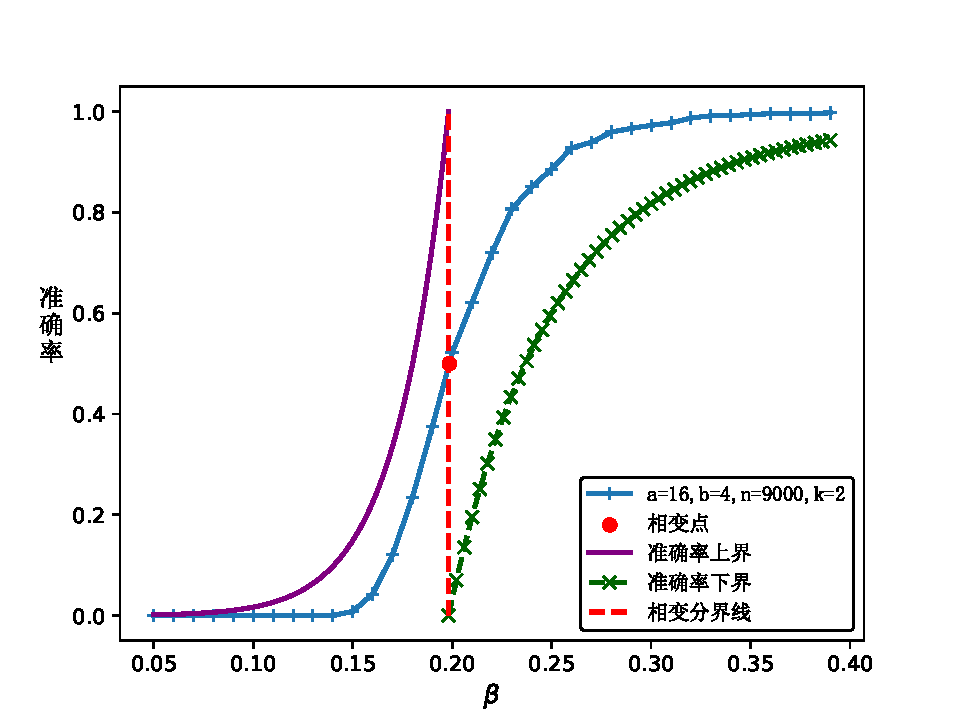
\includegraphics[width=0.6\textwidth]{beta_trans-2020-11-28.pdf}
		\caption{使用 $\hat{X}^*$ 进行社团发现精确恢复的准确率}\label{fig:erh}
\end{figure}


竖线 ($\beta=\beta^* \approx 0.198$),
是 从式 \eqref{eq:beta_star} 计算得到的, 
代表了相变的临界值。
图 \ref{fig:erh} 中的坐标点 $(0.199,\frac{1}{2})$
可视为通过实验估计出的
相变点,它的横坐标接近
$\beta^*$。
绿线 $(\beta, n^{g(\beta)/2})$ 
表示当 $\beta>\beta^*$ 时准确率的理论下界,
而紫线
$(\beta, n^{-g(\beta)})$ 
表示当 $\beta<\beta^*$ 时准确率的理论上界。
仿真实验得到的相变曲线(蓝线)恰好介于这两线之间。
当 $n$ 变得更大时,可预见
相变曲线 将接近阶跃函数,该函数的值在
$\beta=\beta^*$ 处
从 0 跳变到 1。

另外,我们把本节提出的基于玻茨模型的算法应用于实际的网络中。
为了和经典的最大模块度等方法进行公平比较,
我们取超参$\gamma=\gamma_{\mathrm{MQ}}$(参见式\eqref{eq:Qtransform}),
使得$\gamma>b$的条件满足,并且能量函数\eqref{eq:energy}固定下来。
由式\eqref{eq:e_1},$\gamma = \frac{2|E|}{n \log n}$,
故$\gamma$可由输入网络计算。
然后我们通过算法 \ref{alg:m} (Potts) 近似求解能量函数最大值。
该算法与模拟退火的优化策略不同,一旦设定了初始的逆温度参数$\beta$,
$\beta$不随
迭代次数而改变。
在本组实验中我们取$N=40$,$\beta$在
$[1.5,3.0]$的范围内进行超参优化。
我们考虑 Karate\cite{zachary1977information}、
American Football \cite{girvan2002community}、
Dolphin \cite{lusseau2003emergent}
和 Polbooks \cite{newman2006modularity}
四个常用于社团发现算法测试的数据集。
这四个数据集均为有真实标签的无向图。
我们使用归一化的互信息\cite{Danon_2005}作为算法评价指标,
其取值在0到1之间,NMI取1时表明精确恢复。
而我们对比的算法有
Greedy GN \cite{clauset2004finding}、
Fluid \cite{pares2018fluid}、
Louvain \cite{blondel2008fast} 和
标签传播\cite{cordasco2010community}。
实验结果如表 \ref{tab:flatten_result} 所示。
从该表可以看出,我们的算法可以精确恢复 Karate 数据的社团结构,
在其他数据集上也取得不逊于其他算法的结果,从而验证了应用
算法 \ref{alg:m} 在实际网络中进行社团发现的可行性。

\begin{table}[!ht]
    \begin{adjustbox}{width=\columnwidth,center}
    \begin{tabular}{cccccc}
    \hline
    NMI               & Greedy GN & Fluid & Louvain  & 标签传播 & Potts\\
    \hline
    Karate            & 0.692     & 0.837 & 0.587   & 0.445         & 1.000     \\
    American Football & 0.698     & 0.851 & 0.857    & 0.870         & 0.870    \\
    Dolphin           & 0.573     & 0.655 & 0.516    & 0.527        & 0.701     \\
    Polbooks          & 0.531     & 0.411 & 0.493  & 0.534          & 0.580     \\
    \hline
    \end{tabular}
\end{adjustbox}
    \caption{常用社团发现算法在实际网络上的性能比较}\label{tab:flatten_result}
\end{table}

% !TeX root = ../thuthesis-example.tex
\section{定理证明}
\subsection{定理\ref{thm:ab12} 的证明}
\begin{lemma}\label{lem:ER_tr_counting}
  \newglossaryentry{e_r}{name=埃尔德什-雷尼模型, description={Erdős–Rényi model}}
  考虑一个由\gls{e_r}生成的随机图 $G$,它有  $n$
  个节点, 每条边以概率 $p$ 随机生成\cite{erdHos1960evolution}。
   假设
	$p=\A$, 边的数量
  记为  $N_E$ 
  而图中三角形的
  数量记为  $T$。 则
  \newglossaryentry{not:converge_in_probability}
{
  type=notation,
  name={$\xrightarrow{p}$},
  description={随机变量的依概率收敛}
}
	$\frac{N_E}{n \log n} \xrightarrow{p} \frac{a}{2}$ 且
  $\frac{T}{\log^3 n} \xrightarrow{p} \frac{a^3}{6}$。
  这里, 符号 $\xrightarrow{p}$ 表示\glsdesc{not:converge_in_probability}。
\end{lemma}
\begin{proof}
		令 $X_{ij}$ 表示
    参数 为 $p$ 的伯努利随机变量。
    \newacronym{acr:iid}{i.i.d.}{Independent and identically distributed}
    则 $N_E
    = \sum_{i,j} X_{ij}$, $X_{ij}$ 是 \gls{acr:iid}
    的随机变量。
	$\mathbb{E}[N_E] = \frac{n(n-1)}{2}p = \frac{(n-1)\log n}{2}a$ 
  且  $\Var[N_E] = \frac{n(n-1)}{2} p(1-p) < a\frac{(n-1)\log n}{2}$。
	则由切比雪夫不等式,
	\begin{align*}
	P(\Big|\frac{N_E}{n \log n } - \frac{a}{2} \frac{n-1}{n}\Big| > \epsilon) & \leq
	\frac{1}{\epsilon^2}\Var \left[\frac{N_E } {n \log n } \right] \\
	& < \frac{a(n-1)}{2n^2\epsilon^2\log n}
	\end{align*}
	
	对于给定的 $\epsilon$, 当 $n$ 充分大时,
  \begin{align*}
	P \left(\Big|\frac{N_E}{n \log n } - \frac{a}{2} \Big| > \epsilon \right) & <
	P \left(\Big|\frac{N_E}{n \log n } - \frac{a}{2} \frac{n-1}{n}\Big| > 2\epsilon \right) \\
	& \leq \frac{n-1}{8n^2 \epsilon^2 \log n}
	\end{align*}
	
	因此, 由依概率收敛的定义
  我们有 $\frac{N_E}{n \log n} \xrightarrow{p} \frac{a}{2}$。
	
	令 $X_{ijk}$ 表示参数为  $p^3$ 的 Bernoulli 随机变量。
	则 $T = \sum_{i,j,k} X_{ijk}$。
	易得 $\mathbb{E}[T] = \binom{n}{3}p^3$。
  因为 $X_{ijk}$ 并不独立,
  不能直接用独立同分布的公式计算 $T$ 的方差。
	由  \citet{holland1977method} 一文可知:
	% Mordern version: https://stats.stackexchange.com/questions/338267/distribution-and-variance-of-count-of-triangles-in-random-graph
	\begin{align*}
	\Var[T]  &= \binom{n}{3} p^3 + 12 \binom{n}{4} p^5 + 30 \binom{n}{5} p^6 + 20 \binom{n}{6} p^6
	 - \binom{n}{3}^2 p^6  \\ 
   &= O(\log^3 n)
	\end{align*}
	
	因此
	由 切比雪夫不等式可得
	\begin{align*}
	P \left (\Big|\frac{T}{\log^3 n } - \frac{a^3}{6} \frac{(n-1)(n-2)}{n^2}\Big| > \epsilon \right)
   &\leq \frac{1}{\epsilon^2} \Var[ \frac{T}{\log^3 n} ]\\ 
	& = \frac{1}{\epsilon^2}O \left(\frac{1}{\log^3 n} \right)
	\end{align*}
	    
	从而得到 $\frac{T}{\log^3 n} \xrightarrow{p} \frac{a^3}{6}$。
\end{proof}
因为每条边的生成是独立的,埃尔德什-雷尼模型中的
$N_E$ 的收敛性 %define if appropriate.
可以直接拓展到
随机块模型。
但是对于三角形的数量$T$,因为每个三角形存在与否并不独立,事情变得棘手。
下面的两个引理给出了随机块模型中的三角形个数的方差的公式。
\begin{lemma}\label{lem:SBM_tr_counting_cross}
	考虑 $\SSBM(2n, 2, p, q)$。它有两个
  社团,记为 $S_1$ 和 $S_2$。
    计算三角形的个数 $T$, 并且这些三角形
    有一个顶点在  $S_1$ 中,
    该顶点对应的边在 $S_2$中。
   则 $T$ 的方差为:
\begin{align}
\Var[T]  = \frac{n^2(n-1)}{2}pq^2 + n^2(n-1)(n-2)p^2q^3 
 + \frac{n^2(n-1)^2}{2}pq^4 - \frac{n^2(n-1)(3n-4)}{2} p^2 q^4
 \label{eq:SBM_tr_counting_cross}
\end{align}
\end{lemma}
\begin{proof}
	由定义, $T=\sum_{i,j,k} Y_{ijk}$,
  其中 $i,j,k$三个点之间两两有边相连时 $Y_{ijk}$ 取值为1,否则为0。
  这里的求和是
  针对 所有 的 $i \in S_1$ 和 $j,k \in S_2$。
  因此, $\E[T] = n\binom{n}{2}pq^2$。
	为计算 $T$ 我们需要求出 $\E[T^2] = \sum_{i,j,k}\sum_{i',j',k'} Y_{ijk}Y_{i'j'k'}$。
	根据三元组 $(i,j,k)$ 和 $(i',j',k')$ 重合的情况
  $\E[Y_{ijk}Y_{i'j'k'}]$的值一共有6种不同的情形:
	\begin{enumerate}
		\item $\{i,j,k\} = \{i',j',k'\}$,则 $E[Y_{ijk}Y_{i'j'k'}] = pq^2$。
		在 $\E[T^2]$的求和式中共有 $n\binom{n}{2}$ 
     项。以下五种情形均需考虑$\E[T^2]$ 中出现的2倍的系数。
		\item 若 $\{i,j,k\}$ 和 $\{i',j',k'\}$ 只有
    一个共同的元素
    并且这个元素在 $ S_1$ 中, 则 $\E[Y_{ijk}Y_{i'j'k'}] = p^2q^4$。
		在 $\E[T^2]$的求和式中共有 $6n\binom{n}{4}$ 项 ($\binom{4}{2}=6$ )。
		\item 若 $\{i,j,k\}$ 和 $\{i',j',k'\}$ 只有一个共同的元素
    并且这个元素 在 $ S_2$ 中,则
    $E[Y_{ijk}Y_{i'j'k'}] = p^2q^4$。在 $\E[T^2]$的求和式
		中共有 $12\binom{n}{2}\binom{n}{3}$ 项。
		\item 若 $\{i,j,k\}$ 和 $\{i',j',k'\}$ 恰有 2  个 共同的元素
    并且这两个元素均在 $S_2$ 中,
    则 $E[Y_{ijk}Y_{i'j'k'}] = pq^4$。
    在 $\E[T^2]$的求和式
		中共有  $2\binom{n}{2}\binom{n}{2}$ 项。
\item 若 $\{i,j,k\}$ 和 $\{i',j',k'\}$ 恰有2  个 共同的元素
且一个在 $S_1$ 中,另一个在 $S_2$ 中,则 $E[Y_{ijk}Y_{i'j'k'}] = p^2q^3$。
在 $\E[T^2]$的求和式
		中共有 $6n\binom{n}{3}$ 项。
\item  若 $\{i,j,k\}$ 和 $\{i',j',k'\}$ 没有共同的元素,
 则 $E[Y_{ijk}Y_{i'j'k'}] = p^2q^4$。
 在 $\E[T^2]$的求和式中共有 $12\binom{n}{2}\binom{n}{4}$ 
 项。
	\end{enumerate}
通过下面的求和式可以验证我们已经遍历了所有的情形:
% Mathematica Code:
% Simplify[n^2 (n-1)/2 + 12 Binomial[n,2] Binomial[n,3] + 6 n Binomial[n,4] + Binomial[n,4] Binomial[n,2]*12 + 6 n Binomial[n,3]+ 2 Binomial[n,2]^2]
\begin{equation}\label{eq:ver_nn2}
  n\binom{n}{2} + 6n\binom{n}{4} + 12\binom{n}{2} \binom{n}{3} + 2\binom{n}{2}^2 + 6n\binom{n}{3} + 12\binom{n}{2}\binom{n}{4} = \left(n\binom{n}{2}\right)^2  
\end{equation}
\eqref{eq:ver_nn2}式右端中出现的$n\binom{n}{2}$ 是$\E[T] $ 中求和式的项数。
\end{proof}
\begin{lemma}\label{lem:SBM_tr_counting_3}
	考虑 $\SSBM(3n, 3, p, q)$。它有3个社团,记为
  $S_1,S_2$ 和 $S_3$。
  计算三角形的个数 $T$,
  并且这些三角形 有一个顶点在$S_1$中,有一个顶点在 $S_2$中,
  有一个顶点在 $S_3$ 中。
	则 $T$ 的方差为:
	\begin{equation*}\label{eq:SBM_tr_counting_three}
	\Var[T] = n^3 q^3  + 3n^3(n-1) q^4  + 3 n^3 (n-1)^2 q^5 - n^3(3n^2-3n+1)q^6
	\end{equation*}
\end{lemma}

\begin{proof}
	与引理\ref{lem:SBM_tr_counting_cross} 的证明类似,
	$\E[T] = n^3 q^3$,对于$\E[T^2]$求和式中的项共如下4种情形:
	\begin{enumerate}
	\item 若 $\{i,j,k\} = \{i',j',k'\}$, 则 $E[Y_{ijk}Y_{i'j'k'}] = q^3$。
	$\E[T^2]$中 共有 $n^3$ 项。
	\item 若 $\{i,j,k\}$ 和 $\{i',j',k'\}$ 有一个共同的元素, 则 $E[Y_{ijk}Y_{i'j'k'}] = q^5$。
	$\E[T^2]$中 共有 $12n\binom{n}{2}^2$ 项。
	\item 若 $\{i,j,k\}$ and $\{i',j',k'\}$ 有两个共同的元素, 则 $E[Y_{ijk}Y_{i'j'k'}] = q^4$。
	$\E[T^2]$中 共有 $6\binom{n}{2}n^2$ 项。
	\item If $\{i,j,k\}$ and $\{i',j',k'\}$ 没有共同的元素, 则  $E[Y_{ijk}Y_{i'j'k'}] = q^6$。
	$\E[T^2]$中 共有 $8\binom{n}{2}^3$ 项。
\end{enumerate}	
通过下面的求和式可以验证我们已经遍历了所有的情形:
$$
6\binom{n}{2}n^2  + 8\binom{n}{2}^3 + 12n\binom{n}{2}^2 +  n^3 = n^6
$$
\end{proof}
\begin{lemma}\label{lem:sbmV}
 对于 $\SSBM(n, k, p, q)$,其中 $p=\frac{a\log n}{n}, q = \frac{b\log n}{n}$。
 三角形的数量为 $T$。
	则 $\frac{T}{(\log n)^3}$ 依概率收敛到 $\frac{1}{k^2}(\frac{a^3}{6} + \frac{k-1}{2}ab^2 + (k-1)(k-2)\frac{b^3}{6} )$。
\end{lemma}
\begin{proof}
 我们将 $T$ 分成三部分:
 第一部分是每个社团内部的三角形,记社团$i$里有$T_i$个三角形,则共有$k$个$T_i$的项。
 第二部分包括有一个点在第i个社团内部,它所对的边在第$j$个社团里的那些三角形,记为 $T_{ij}$。
 共有 $k(k-1)$ 个 $T_{ij}$ 的项。第三部分包括三个顶点分别在$i,j,k$三个不同社团的三角形,共有
 $\binom{n}{3}$ 项。
	
	我们只需证明:
\begin{align}
	\frac{T_i}{\log ^3 n} &\xrightarrow{p} \frac{(a/k)^3}{6} \\
	\frac{T_{ij}}{\log^3 n}& \xrightarrow{p}\frac{1}{2}(a/k)(b/k)^2\\
	\frac{T_{ijk}}{\log^3 n} & \xrightarrow{p} (b/k)^3
	\end{align}
	
	$\frac{T_i}{\log ^3 n}$ 的收敛性可以直接从引理
 \ref{lem:ER_tr_counting} 中得到。这里,我们视$p=\frac{(a/k) (
    \log (n/k) + \log k)}{(n/k)}$,因为 $\log k$ 相比于其前一项量阶更小,
    可以忽略不计。
	对于 $T_{ij}$, 我们使用 
  引理\ref{lem:SBM_tr_counting_cross} 的结果。
	在 \eqref{eq:SBM_tr_counting_cross} 式中
  我们用 $n/k$ 代替 $n$, 取 $p=a\frac{\log n}{n}$ 且 $q=b\frac{\log n}{n}$。
	$\Var[T_{ij}] \sim \frac{ab^2}{2k^3} \log^3 n$。
  因为 $\frac{T_{ij}}{\log^3 n}$ 的期望值是
  $(n/k)\binom{n/k}{2}pq^2/(\log^3 n)
	=\frac{n-1}{2n}\frac{ab^2}{k^3}$, 由切比雪夫不等式
  可得:
	\begin{align*}
	P \left( \Big|\frac{T_{ij}}{\log^3 n} - \frac{n-1}{2n}\frac{ab^2}{k^3} \Big| > \epsilon
  \right) &\leq \frac{\Var[T_{ij} / \log^3 n]}{\epsilon^2} \\
	& = \frac{1}{\epsilon^2}
	O \left( \frac{1}{\log^3 n} \right)
	\end{align*}
	
	因此, $\frac{T_{ij}}{\log^3 n} $ 依概率收敛到 $\frac{1}{2}(a/k)(b/k)^2$。
	
	为证明
  $\frac{T_{ijk}}{\log^3 n}\to (b/k)^3$,
  从 引理\ref{lem:SBM_tr_counting_3} 中
  可得 $\Var[T_{ijk}] = O(\log^5 n)$:
	$$
	P \left( \Big|\frac{T_{ijk}}{\log^3 n} -\frac{b^3}{k^3} \Big| > \epsilon
  \right) \leq \frac{\Var[T_{ijk} / \log^3 n]}{\epsilon^2} = \frac{1}{\epsilon^2}
	O \left(\frac{1}{\log n} \right)
	$$
\end{proof}
\begin{proof}[定理\ref{thm:ab12} 的证明]
	令 $e^*_1 = \frac{a+(k-1)b}{2k}$, $k^2 e^*_2 = \frac{a^3}{6} + \frac{k-1}{2}ab^2 + (k-1)(k-2)\frac{b^3}{6}$
	且 $e_1 = \frac{T_1}{n\log n}, e_2 = \frac{T_2}{\log^3 n}$。
	由 引理
 \ref{lem:ER_tr_counting}, $e_1 \to e^*_1$。
	由 引理\ref{lem:sbmV}, 当 $n\to \infty$ 时,
  $e_2 \to e^*_2$。
	通过变量替换 $x=2ke_1 - (k-1)y$ 消元,我们可将
  方程组 (\ref{eq:e_1},\ref{eq:e_2})
  化简为如下的非线性方程:
\begin{equation}\label{eq:gy_y3}
g(y): = (k-1)(y^3 - 6 e_1 y^2 + 12 e_1^2 y) + 6 e_2 - 8 k e_1^3 = 0
\end{equation}

$g'(y) = 3(k-1)(y-2e_1)^2 \geq 0 $,
$g(y)$ $\mathbb{R}$上的是增函数,
因此方程\eqref{eq:gy_y3} 最多有一个实根。
下面我们证明\eqref{eq:gy_y3}式有一个实根
在 区间 $(0, 2e_1)$ 内。
\begin{align*}
&\lim_{n\to \infty}g(0) =  6e^*_2 - 8k(e^*_1)^3 =-\frac{3}{k^2}(k-1)(k-2)ab^2 \\
&-\frac{3(k-1)}{k^2}a^2b - \frac{k-1}{k^2} ((k-2)-(k-1)^2)b^3 < 0 \\
&\lim_{n\to \infty}g(2e_1) = 6e^*_2 - 8(e^*_1)^3 = \frac{(k-1)(a-b)^3}{k^3} > 0
% verified with sympy
\end{align*}

因此,\eqref{eq:gy_y3}式有一个实根,由 $g(y)$的连续性,当$n\to \infty $ 时,该实根收敛到 $b$。
从而我们得到方程组 (\ref{eq:e_1},\ref{eq:e_2})有唯一解 $\hat{a},\hat{b}$,
且
$\hat{b} \to b$, $\hat{a} \to a$。
\end{proof}

\subsection{引理\ref{lem:lemmaDiff}的证明}

\begin{proof}[引理\ref{lem:lemmaDiff}的证明]
	首先我们将
  \eqref{eq:energy} 式改写成
	\begin{equation*}
	H(\bar{\sigma}) = \gamma \frac{\log n}{n} \sum_{i < j} \delta(\bar{\sigma}_i, \bar{\sigma}_j)
	- (1 + \gamma\frac{\log n}{n}) \sum_{ \{i, j\} \in E(G)} \delta(\bar{\sigma}_i, \bar{\sigma}_j)
	\end{equation*}
	
	接着我们逐步计算能量差:
  \begin{align*}
	H(\bar{\sigma}') - H(\bar{\sigma}) =& 
  \left(1 + \gamma\frac{\log n}{n}
  \right)
  \cdot \sum_{i \in N_r(G)} (\delta(\bar{\sigma}_r, \bar{\sigma}_i) -
	\delta(\omega^s \cdot \bar{\sigma}_r, \bar{\sigma}_i)) \\
	&+ \gamma \frac{\log n}{n}\sum_{i\neq r}
	( \delta(\omega^s \cdot \bar{\sigma}_r, \bar{\sigma}_i) -
	\delta( \bar{\sigma}_r, \bar{\sigma}_i) ) \\
	 =& \left(
     1 + \gamma\frac{\log n}{n}
     \right)
   \sum_{i \in N_r(G)} J_s(\bar{\sigma}_r, \bar{\sigma}_i) \\
	&+ \gamma \frac{\log n}{n}\sum_{i=1}^n
	( \delta(\omega^s \cdot \bar{\sigma}_r, \bar{\sigma}_i) -
	\delta( \bar{\sigma}_r, \bar{\sigma}_i) +1) \\
	=& \left(1+\gamma \frac{\log n}{n}
  \right)
  \sum_{i \in N_r(G)} J_s(\bar{\sigma}_r, \bar{\sigma}_i)\\
	&+ \gamma \frac{\log n}{n} (m(\omega^s \cdot \bar{\sigma}_r)-m(\bar{\sigma}_r)+1)
	\end{align*}
\end{proof}

\subsection{定理\ref{thm:phase_transition}的证明}
\label{sec:appendix_theorem_proof_phase_trans}

在开始定理\ref{thm:phase_transition}的技术证明之前,
我们需要介绍一些辅助的
符号。

% Some additional notation is needed for the proof.
注释\ref{re:energy_diff}中指出了
$X$改变一个状态后的能量差表达式。
对于一般的情形,即改变
$|\cI|:=\Dist(\bar{\sigma}, X)$
个位置的状态后,
我们可以将能量差写成:
\begin{equation}\label{eq:Hgeneral}
H(\bar{\sigma}) - H(X)=
(1 + \gamma \frac{ \log n}{n})[A_{\bar{\sigma}} - B_{\bar{\sigma}}] + \gamma\frac{ \log n}{n} N_{\bar{\sigma}}
\end{equation}
在上式中 我们使用
$A_{\bar{\sigma}}$ 或
$B_{\bar{\sigma}}$ 来表示
服从参数分别为 $\A$ 或 $\B$ 的二项分布的随机变量,并且
$N_{\bar{\sigma}}$ 是一个依赖于 $\bar{\sigma}$ 但与图结构无关的非随机的正整数。
引理\ref{lem:minus} 给出了 $A_{\bar{\sigma}}, B_{\bar{\sigma}}$ 和 $N_{\bar{\sigma}}$
的表达式:

\begin{lemma}\label{lem:minus}
	对于 $\SSBM(n,k,p,q)$,
  我们假设 $\bar{\sigma}$ 
  在总共$|\cI|:=\Dist(\bar{\sigma}, X)$ 
  个坐标位置上不同于真值标签向量
  $X$。
	对于 $i\neq j$,令 $I_{ij} = \Big|\{r\in [n] \big| X_r = w^i, \sigma_r = w^j \}\Big|$
  且 $I_{ii} = 0$。
  我们进一步将行和$I_i$
  和列和$I'_i$分别表示为:
  \begin{align}
  I_i &= \frac{n}{k} -
  \Big|\{r\in [n] \big| X_r = w^i, \sigma_r=w^i \}\Big|
  =
  \sum_{j=0}^{k-1} I_{ij} \label{eq:I_i_horizontal} \\
  I'_i &=
  \Big|\{r\in [n] \big| X_r \neq w^i,
  \sigma_r=w^i \}\Big|
  =\sum_{j=0}^{k-1} I_{ji}\label{eq:I_prime_i_vertical}
  \end{align}
	则
\begin{align}
	N_{\bar{\sigma}} &= \frac{1}{2}\sum_{i=0}^{k-1} (I_i - I_i')^2 \label{eq:N_w} \\
	B_{\bar{\sigma}} & \sim \Binom(N_{B_{\bar{\sigma}}} , q),
  N_{B_{\bar{\sigma}}}=\frac{n}{k}|\cI| + \frac{1}{2}\sum_{i=0}^{k-1}  (-2 I'_i I_i  + I'^2_i - \sum_{j=0}^{k-1} I^2_{ji})
  \label{eq:B_w}\\
	A_{\bar{\sigma}} &
  \sim \Binom(N_{A_{\bar{\sigma}}}, p),
  N_{A_{\bar{\sigma}}}=
  \frac{n}{k}|\cI| - \frac{1}{2}\sum_{i=0}^{k-1}
   (I^2_i + \sum_{j=0}^{k-1} I^2_{ij})
  \label{eq:A_w}
	\end{align}
\end{lemma}
\begin{proof}
  由式\eqref{eq:isingma}、\eqref{eq:energy}可得
	\begin{align}
  \log P_{\sigma|G}(\sigma=\bar{\sigma})
  & = 
  \beta(1 + \frac{\gamma \log n}{n}) \sum_{\{i,j\} \in E(G)}  \delta(\bar{\sigma}_i, \bar{\sigma}_j)  
	- \beta\frac{\gamma \log n}{n} \sum_{1\leq i<j \leq n} \delta(\bar{\sigma}_i, \bar{\sigma}_j)  - \log Z_G(\beta, \gamma)
  \notag\\
  & = 
  \beta(1 + \frac{\gamma \log n}{n}) \sum_{\bar{\sigma}_i = \bar{\sigma}_j} Z_{ij}
	- \beta\frac{\gamma \log n}{n}
  \sum_{\bar{\sigma}_i = \bar{\sigma}_j} 1 
  - \log Z_G(\beta, \gamma)
  \label{eq:log_P_sigma_G_bar_sigma}
  \end{align}
	其中 $Z_{ij}$ 服从伯努利分布,
  $P(Z_{ij}=1)$ 等于节点$i$与节点$j$之间有边相边的概率。
	对于 $\sigma = X$, 我们有
	\begin{align}
	\sum_{X_i = X_j} Z_{ij} &
  = \sum_{X_i = X_j, \bar{\sigma}_i = \bar{\sigma}_j}
  Z_{ij} + \sum_{X_i = X_j, \bar{\sigma}_i \neq \bar{\sigma}_j}
  Z_{ij}
  \label{eq:split_zij_tmp_X_ij}\\
	\sum_{X_i = X_j} 1 &= \frac{1}{2} \sum_{i=0}^{k-1} \frac{n}{k} 
  \left( \frac{n}{k} - 1 
  \right)\label{eq:split_one_tmp_X_ij}
	\end{align}
	对于 $\sigma = \bar{\sigma}$,我们有
	\begin{align}
	\sum_{\bar{\sigma}_i = \bar{\sigma}_j} Z_{ij} &= \sum_{X_i = X_j, \bar{\sigma}_i = \bar{\sigma}_j} Z_{ij} + \sum_{X_i \neq X_j, \bar{\sigma}_i = \bar{\sigma}_j} Z_{ij} 
  \label{eq:split_zij_tmp_sigma_ij}\\
	\sum_{\bar{\sigma}_i = \bar{\sigma}_j} 1 &= \frac{1}{2} \sum_{i=0}^{k-1} (I'_i + \frac{n}{k} - I_i) ( I'_i + \frac{n}{k} - I_i - 1)
  \label{eq:split_one_tmp_sigma_ij}
	\end{align}
  其中,式 \eqref{eq:split_one_tmp_sigma_ij} 是根据式
  \eqref{eq:I_i_horizontal}和 \eqref{eq:I_prime_i_vertical}
  而来。
	注意到
  $
  \Big|\{r\in [n] \big| X_r = w^i, \sigma_r=w^i \}\Big|
  =\frac{n}{k} - I_i$和
	$|\{r\in [n] | X_r \neq \omega^i, \sigma_r = \omega^i \}| = I'_i$,
	我们因此有  
  \begin{equation}\label{eq:number_of_sigma_r_equal_omega_i}
    |\{r\in [n] | \sigma_r = \omega^i \}|
    = I'_i + \frac{n}{k} - I_i
  \end{equation}
  类比式\eqref{eq:split_one_tmp_X_ij}从而得到
  式\eqref{eq:split_one_tmp_sigma_ij}。

  由式\eqref{eq:Pratio} 我们得到
  \begin{equation}
    \frac{P_{\sigma |G } (\sigma = \bar{\sigma})}
    {P_{\sigma |G } (\sigma = X)}
    = \exp(-\beta(H(\bar{\sigma})
    - H(X)))
  \end{equation}
  结合式\eqref{eq:log_P_sigma_G_bar_sigma}
  可得
  \begin{equation}\label{eq:Hgeneral_tmp_derived}
    H(\bar{\sigma}) - H(X)=
    -\left(1 + \gamma \frac{ \log n}{n}
    \right)
    \left[
      \sum_{\bar{\sigma}_i = \bar{\sigma}_j}Z_{ij} - \sum_{X_i = X_j}Z_{ij}
      \right]
    + \gamma\frac{ \log n}{n}
    \left[\sum_{\bar{\sigma}_i = \bar{\sigma}_j}1 - \sum_{X_i = X_j}1
    \right]
    \end{equation}
  将式\eqref{eq:Hgeneral_tmp_derived} 与式\eqref{eq:Hgeneral}
  对比可得:
  \begin{align}
    B_{\bar{\sigma}} - A_{\bar{\sigma}} &=
    \sum_{\bar{\sigma}_i = \bar{\sigma}_j}Z_{ij}
    - \sum_{X_i = X_j}Z_{ij}
    \label{eq:B_bar_A_bar_lem_minus}\\
    N_{\bar{\sigma}} &=
    \sum_{\bar{\sigma}_i = \bar{\sigma}_j} 1  -\sum_{X_i = X_j} 1
    \label{eq:N_bar_sigma_lem_minus}
  \end{align}
  由式\eqref{eq:split_one_tmp_X_ij},
  \eqref{eq:split_one_tmp_sigma_ij}, 
  \eqref{eq:N_bar_sigma_lem_minus} 可得
  $N_{\bar{\sigma}} = \sum_{\bar{\sigma}_i = \bar{\sigma}_j} 1  -\sum_{X_i = X_j} 1 = \frac{1}{2}\sum_{i=0}^{k-1} (I_i - I_i')^2 $,
  即式 \eqref{eq:N_w}。
	另一方面,由式\eqref{eq:B_bar_A_bar_lem_minus},
  \eqref{eq:split_zij_tmp_X_ij}, 
  \eqref{eq:split_zij_tmp_sigma_ij}
  可得 $B_{\bar{\sigma}} - A_{\bar{\sigma}} = \sum_{X_i \neq X_j, \bar{\sigma}_i = \bar{\sigma}_j} Z_{ij} - \sum_{X_i = X_j, \bar{\sigma}_i \neq \bar{\sigma}_j} Z_{ij}$。
	对于在求和式 $\sum_{X_i \neq X_j, \bar{\sigma}_i = \bar{\sigma}_j} Z_{ij}$
  中出现的 $Z_{ij}$, $Z_{ij} \sim \Bern(q)$
  并且我们有
  \begin{align}
  \sum_{X_i \neq X_j, \bar{\sigma}_i = \bar{\sigma}_j} 1 
  &= \sum_{i=0}^{k-1}[(\frac{n}{k} - I_i) I_i' + \frac{1}{2} \sum_{j=0}^{k-1} I_{ji}(I'_i - I_{ji}) ] 
  \label{eq:x_i_neq_x_j_bar_sigma_i_eq_bar_sigma_j_0}\\
	&=\frac{n}{k}|\cI| + \frac{1}{2}\sum_{i=0}^{k-1}  (-2 I'_i I_i  + I'^2_i - \sum_{j=0}^{k-1} I^2_{ji}) 
  \label{eq:x_i_neq_x_j_bar_sigma_i_eq_bar_sigma_j_1}
  \end{align}
  在式\eqref{eq:x_i_neq_x_j_bar_sigma_i_eq_bar_sigma_j_0}
  最外层的求和中,首先遍历的是$X_i=1, \omega, \dots, \omega^{k-1}$。  
  而式\eqref{eq:split_one_tmp_sigma_ij}
  利用了
  $|\cI| = \sum_{i=0}^{k-1} I'_i$。
  类似的,
  对于在求和式 $\sum_{X_i = X_j, \bar{\sigma}_i \neq \bar{\sigma}_j} Z_{ij}$
  中出现的 $Z_{ij}$, $Z_{ij} \sim \Bern(p)$。
	$\sum_{X_i = X_j, \bar{\sigma}_i \neq \bar{\sigma}_j} 1
	= \sum_{i=0}^{k-1}[(\frac{n}{k} - I_i) I_i + \frac{1}{2} \sum_{j=0}^{k-1} I_{ij}(I_i - I_{ij}) ] 
	= \frac{n}{k}|\cI| - \frac{1}{2}\sum_{i=0}^{k-1}  (I^2_i + \sum_{j=0}^{k-1} I^2_{ij})$。
  从而式\eqref{eq:B_w}、\eqref{eq:A_w} 得证。
\end{proof}

从上面可以看到引理\ref{lem:minus} 的证明并没有很多技巧性,主要涉及一些计数
的技巧。
当 $|\cI|$ 相比与 $n$ 很小时
我们有如下的引理, 该引理是 \citet{ye2020exact} 中 陈述 6 的拓展。 

\begin{lemma}
  \label{lem:enhanced_fb}
	对于 $t\in [\frac{1}{k}(b-a), 0], 0<\delta <1$
	和 $ |\cI| \le n/\log^{\delta} n$,我们有
\begin{equation} \label{eq:upmpt}
	P_G(B_{\bar{\sigma}}-A_{\bar{\sigma}}\ge t |\cI| \log n) 
	\le  \exp\Big(|\cI|\log n
	\left(
    f_{\beta}(t) - \beta t -1	+ O((\log n)^{-\delta}) \right)\Big)
	\end{equation}
	其中 $f_{\beta}(t) := \min_{s\geq 0} (g(s) - st) + \beta t \leq \tilde{g}(\beta) $。
  $P_G$中的下标$G$表示图$G$是由SSBM模型随机生成的。
  函数$g(\beta), \tilde{g}(\beta)$
  的定义分别参见
  \eqref{eq:g_beta_main_article}
  和
  \eqref{eq:g_tilde_beta_main_article} 式。
\end{lemma}

在引理\ref{lem:enhanced_fb} 中,
取
$|\cI|=1, N_{\bar{\sigma}}=0$,
此时$A_{\bar{\sigma}} \sim \Binom(\frac{n}{k}, \A),
B_{\bar{\sigma}} \sim \Binom(\frac{n}{k}, \B)$,
即得到 式\eqref{eq:introduction_g_a_b_eps}。

\begin{proof}[引理\ref{lem:enhanced_fb} 的证明]
  由$f_{\beta}(t)$函数的定义,
  \eqref{eq:upmpt}式中
  $f_{\beta}(t) - \beta t$ 与$\beta$无关而只与
  $t$有关。
	由定义可知,
  $A_{\bar{\sigma}}\sim \Binom(N_{A_{\bar{\sigma}}},\frac{a\log n}{n})$
  且
	$B_{\bar{\sigma}}\sim\Binom(N_{B_{\bar{\sigma}}},\frac{b\log n}{n})$,
  并且二者彼此独立。
  由 (\ref{eq:N_w}-\ref{eq:A_w})可知,$N_{B_{\bar{\sigma}}} - N_{A_{\bar{\sigma}}}
  = N_{\bar{\sigma}}$。
  对于$s>0$,
  $B_{\bar{\sigma}}-A_{\bar{\sigma}}$ 的矩生成函数可以展开成
	\begin{align}
	 \mathbb{E}[e^{s(B_{\bar{\sigma}}-A_{\bar{\sigma}})}] 
	& =\Big(1-\frac{b\log n}{n}+\frac{b\log n}{n} e^s \Big)^{N_{B_{\bar{\sigma}}}}
	\Big(1-\frac{a\log n}{n}+\frac{a\log n}{n} e^{-s} \Big)^{N_{A_{\bar{\sigma}}}}  \notag\\
	& = \exp\left(\frac{\log n}{n}\left(N_{B_{\bar{\sigma}}}
  (be^s - b) + N_{A_{\bar{\sigma}}}(ae^{-s}-a) + N_{B_{\bar{\sigma}}}
  O \left(\frac{\log n}{n} \right) \right) \right)
  \label{eq:exp_s_B_A_sigma}
	\end{align}
	由\eqref{eq:B_w}
  和\eqref{eq:A_w}
  注意到$k$是个常数,
  当
  $|\cI| \le n/\log^{\delta}(n)$ 时
	我们能估计
  $N_{B_{\bar{\sigma}}}$和$N_{A_{\bar{\sigma}}}$
  的阶数。它们分别是
  $N_{A_{\bar{\sigma}}} = \frac{n}{k}|\cI| + O(|\cI|^2)$,
	 $N_{B_{\bar{\sigma}}} = \frac{n}{k}|\cI| + O(|\cI|^2)$。
	\begin{align*}
	\mathbb{E}[e^{s(B_{\bar{\sigma}}-A_{\bar{\sigma}})}]
   \le&
	\exp(\frac{\log n}{n}\Big((\frac{n}{k}|\cI| + O(|\cI|^2))(be^s - b) +(\frac{n}{k} |\cI| + O(|\cI|^2))(ae^{-s}-a) \\
  &+ \frac{n}{k}|\cI|O(\frac{\log n}{n}) \Big))\\
	=
  & \exp\Big(\frac{|\cI| \log n}{k}(a e^{-s}+b e^s-a-b +
	O(\log^{-\delta}(n))) \Big),
	\end{align*}
	最后一个等式来自于
  $ |\cI| \le n/\log^{\delta}(n)$这个假设。
	由切尔诺夫不等式(参见 \eqref{eq:chernoff_bound}),
  对于 $s>0$,我们有
	\begin{align*} 
	& P_G(B_{\bar{\sigma}}-A_{\bar{\sigma}}\ge t |\cI| \log n)\le
	\frac{\mathbb{E}[e^{s(B_{\bar{\sigma}}-A_{\bar{\sigma}})}]}{e^{st |\cI|  \log n}}  \\
	\le & \exp\Big(\frac{|\cI|\log n}{k} \big(a e^{-s}+b e^s -kst -a-b
	+ O(\log^{-\delta}(n)) \big)\Big)  .
	\end{align*}
	上式右端对$s\geq 0$取最小值即有
  \eqref{eq:upmpt}。  
	\end{proof}

  对应于定理\ref{thm:phase_transition} 的三种情况,我们需要使用若干个非平凡的引理来辅助证明。

  \begin{lemma}\label{lem:sigmaX}
    令 $\gamma > b$, 且 $\bar{\sigma}$ 满足 $\Dist(\bar{\sigma}, X) \geq \frac{n}{\sqrt{\log n}}$
    和 $D(\bar{\sigma}, X)$
    (参见\eqref{eq:D_sigma_sigma_prime})
    两个条件。
    事件
    $P_{\sigma | G}(\sigma = \bar{\sigma} ) > \exp(-Cn) P_{\sigma | G}(\sigma = X)$
    发生的概率小于 $\exp(-\tau(\beta, \gamma) n \sqrt{\log  n} )$,
    其中 $C$ 是任意事先给定的常数而 
    $\tau(\beta, \gamma)$
   是某个依赖于$\gamma$ 和 $\beta$的取值为正值的函数。
  \end{lemma}
  \begin{proof}
    我们把 事件 $P_{\sigma | G}(\sigma = \bar{\sigma} ) > \exp(-Cn) P_{\sigma | G}(\sigma = X)$
    记为 $\widetilde{D}(\bar{\sigma}, C)$。
    由 \eqref{eq:Hgeneral} 式, $\widetilde{D}(\bar{\sigma}, C)$
    等价于:
  \begin{equation}\label{eq:BwA}
    (1 + \frac{\gamma \log n}{n})[B_{\bar{\sigma}} - A_{\bar{\sigma}}] >  \frac{\gamma \log n}{n} N_{\bar{\sigma}}  - \frac{C}{\beta} n
    \end{equation}  
    
    我们声称$\bar{\sigma}$  必须满足以下两个条件中的至少一个。
    \begin{enumerate}
      \item $\exists i\neq j$ s.t. $\frac{1}{k(k-1)}\frac{n}{\sqrt{\log n}} \leq I_{ij} \leq \frac{n}{k} - \frac{1}{k(k-1)}\frac{n}{\sqrt{\log n}}$
      \item $\exists i \neq j$ s.t. $I_{ij} > \frac{n}{k} - \frac{1}{k(k-1)}\frac{n}{\sqrt{\log n}}$ and $I_{ji} < \frac{1}{k(k-1)}\frac{n}{\sqrt{\log n}}$
    \end{enumerate}
    $I_{ij}$的定义参见引理
   \ref{lem:minus}。
    如果上面两个条件均不成立,则由条件1,对 $0 \leq i,j\leq k-1$,
    我们有
    $I_{ij} < \frac{1}{k(k-1)}\frac{n}{\sqrt{\log n}}$
    或者 $I_{ij} > \frac{n}{k} - \frac{1}{k(k-1)}\frac{n}{\sqrt{\log n}}$。
    
    因为 $\sum_{i,j} I_{ij} = |\cI| \geq \frac{n}{\sqrt{\log n}}$,
    存在 $i,j$ 使得
    $I_{ij} > \frac{n}{k} - \frac{1}{k(k-1)}\frac{n}{\sqrt{\log n}}$.
    对于这一对确定的 $i,j$,不妨先假设 $I_{ji} > \frac{n}{k} - \frac{1}{k(k-1)}\frac{n}{\sqrt{\log n}}$,
    下面我们将推出一对矛盾说明该假设不成立。
    取 $X'$ 为在$X$ 的基础上交换$w^i$ 和 $w^j$ 位置的向量,
    然后我们考虑
  \begin{align}
     \Dist(\bar{\sigma}, X') & - \Dist(\bar{\sigma}, X)= |\{ r \in [n]|X_r=w^i, \bar{\sigma}_r \neq w^j \}| \notag\\
    &+ |\{ r \in [n]|X_r=w^j, \bar{\sigma}_r \neq w^i \}| \notag\\
    &-|\{ r \in [n]|X_r=w^i, \bar{\sigma}_r \neq w^i \}| \notag\\
    &- |\{ r \in [n]|X_r=w^j, \bar{\sigma}_r \neq w^j \}| \notag\\
    & = \frac{n}{k} - I_{ij} +  \frac{n}{k} - I_{ji} - I_i - I_j\label{eq:distsmall} \\
    & < \frac{2}{k(k-1)}\frac{n}{\sqrt{\log n}} - I_i - I_j < 0\notag
    \end{align}
    这和 $\bar{\sigma}$ 离 $X$ 最近的条件矛盾。
    因此
    $I_{ji} > \frac{n}{k} - \frac{1}{k(k-1)}\frac{n}{\sqrt{\log n}}$
    不成立,由条件1
    则有  $I_{ji} < \frac{1}{k(k-1)}\frac{n}{\sqrt{\log n}}$。
    但这样一来 $(i, j)$ 二元组满足 条件 2,
    又与 $\bar{\sigma}$ 不满足如上两个条件的假设相矛盾。
    
    在条件1的假设下,我们能获得 $N_{A_{\bar{\sigma}}}$的一个下界。
    为方便估计该下界,我们首先改写\eqref{eq:A_w}式。
    对于 $i\neq j$ ,令 $I'_{ij} = I_{ij}$,
    而 $I'_{ii} = \frac{n}{k} - I_i$。
    则我们有:
    \begin{align*}
    N_{A_{\bar{\sigma}}} &=
    \frac{n}{k}|\cI| - \frac{1}{2}\sum_{i=0}^{k-1}
    (I^2_i + \sum_{j=0}^{k-1} I^2_{ij}) \\
    &=
    \frac{n}{k}|\cI| - \frac{1}{2}\sum_{i=0}^{k-1}
    ((\frac{n^2}{k^2} - 2\frac{n}{k} I'_{ii}) +
    \sum_{j=0}^{k-1} I'^2_{ij}) \\
    &=
    \frac{n}{k}|\cI| - \frac{1}{2}\sum_{i=0}^{k-1}
    ((\frac{n^2}{k^2} - 2\frac{n}{k} (\frac{n}{k} - I_i)))
    - \frac{1}{2}\sum_{i=0}^{k-1}\sum_{j=0}^{k-1} I'^2_{ij} \\
    &= \frac{n^2}{2k} - \frac{1}{2}
    \sum_{i=0}^{k-1} \sum_{j=0}^{k-1} I'^2_{ij}
   \end{align*}
    
    在求和式中 $\sum_{i=0}^{k-1} \sum_{j=0}^{k-1} I'^2_{ij}$
    的每一项 $\sum_{j=0}^{k-1} I'^2_{ij}$ 其满足 $\sum_{j=0}^{k-1}
    I'_{ij} = \frac{n}{k}$,当某个$I'_{ii}$取$\frac{n}{k}$
    而其余的项为零时$\sum_{j=0}^{k-1} I'^2_{ij}$
    最大。但由于条件1成立,有某一行不能取
    这种极端值,所以 $\sum_{i=0}^{k-1} \sum_{j=0}^{k-1} I'^2_{ij}$中
    共有 $(k-1)$行求和得$ (k-1)\frac{n^2}{k^2}$
    而其中一行则必须保留$I'_{ij}, I'_{ii}$ 这两个非零项。
    因此 $\sum_{i=0}^{k-1} \sum_{j=0}^{k-1} I'^2_{ij}
    \leq (k-1)\frac{n^2}{k^2} + (\frac{n}{k} - I_{ij})^2 + I^2_{ij}$。
    而这里的
    $I_{ij}$ 满足条件1。
    进一步的, $\sum_{i=0}^{k-1} \sum_{j=0}^{k-1} I'^2_{ij} \leq (k-1)\frac{n^2}{k^2} + (\frac{1}{k(k-1)}\frac{n}{\sqrt{\log n}})^2
    + (\frac{n}{k} - \frac{1}{k(k-1)}\frac{n}{\sqrt{\log n}})^2 = \frac{n^2}{k} - \frac{2n^2}{k^2 (k-1)\sqrt{\log n}}(1+o(1))$。
    从而我们得到
  \begin{equation}\label{eq:Asigma}
    A_{\bar{\sigma}} \geq \frac{n^2}{k^2 (k-1)\sqrt{\log n}}(1+o(1))
    \end{equation}
    
    
    在条件2的假设下, 我们能得到
    $N_{\bar{\sigma}}$的一个下界。
    因为
    $\Dist(\bar{\sigma}, X') - \Dist(\bar{\sigma}, X) \geq 0$,
     由 \eqref{eq:distsmall} 式 我们有
    $I_{ij} + I_{ji} + I_{i} + I_j \leq \frac{2n}{k} $。
    又因为 $I_i \geq I_{ij} > \frac{n}{k} - \frac{1}{k(k-1)}\frac{n}{\sqrt{\log n}}$,
    从而$I_j $ 满足
    $I_j \leq \frac{2}{k(k-1)}\frac{n}{\sqrt{\log n} }$。
    进一步有 $I'_j - I_j \geq I_{ij} - I_j \geq  \frac{n}{k} - \frac{3}{k(k-1)}\frac{n}{\sqrt{\log n} }$。
    由 \eqref{eq:N_w}
    式 $N_{\bar{\sigma}} \geq \frac{1}{2}(\frac{n}{k} - \frac{3}{k(k-1)}\frac{n}{\sqrt{\log n}})^2 = \frac{n^2}{2k^2}(1+o(1))$.
    
    下面我们用
     切尔诺夫不等式给出\eqref{eq:BwA}式描述的事件发生概率的上界。
     在分析中我们可以省略不等号左边的 $\frac{\gamma \log n}{n}$ 一项
     ,因为其远小于$1$。
    令 $Z \sim \Bern(\A), Z' \sim \Bern(\B)$,则:
    \begin{align*}
    &P_G(\widetilde{D}(\bar{\sigma}, C))
    \leq (\mathbb{E}[\exp(sZ')])^{N_{B_{\bar{\sigma}}}}
    (\mathbb{E}[\exp(-sZ)])^{N_{A_{\bar{\sigma}}}}\\
    &\cdot \exp(-s(\frac{\gamma \log n}{n} N_{\bar{\sigma}}  - \frac{C}{\beta}n)) \\
    & \leq \exp\Big(N_{B_{\bar{\sigma}}}
    \frac{b\log n}{n}(e^s -1) + N_{A_{\bar{\sigma}}}\frac{a\log n}{n} (e^{-s} - 1) \\
    &-s(\frac{\gamma \log n}{n} N_{\bar{\sigma}}  - \frac{C}{\beta}n)\Big) 
    \end{align*}
    
    使用 $N_{B_{\bar{\sigma}}} = N_{\bar{\sigma}} + N_{A_{\bar{\sigma}}}$
    我们可以进一步简化上式中的指数项为:
    $$
    \frac{\log n}{n} [N_{A_{\bar{\sigma}}}(b(e^s -1)+ a(e^{-s} - 1)) +
    N_{\bar{\sigma}} (b(e^s - 1)-\gamma s)]  + s \frac{C}{\beta}n
    $$
    
    下面我们考察 函数 $g_1(s) = b(e^s -1)+ a(e^{-s} - 1)$
    和 $g_2(s) = b(e^s - 1)-\gamma s$。
    两个函数 在 $s=0$ 处取值为零
    并且 $g_1'(s) = (be^s - ae^{-s}), g_2'(s) = be^s -\gamma$。
    因此, $g_1'(0) = b-a<0, g_2'(0) = b - \gamma < 0$
    我们可以选择 $s^*>0$,使得 $g_1(s^*) < 0,g_2(s^*) < 0$。
    为了补偿 $sCn/\beta$ 这一项的影响,我们只需要确保
    $\frac{\log n}{n} \min\{N_{A_{\bar{\sigma}}}, N_{\bar{\sigma}}\}$ 的阶次大于$n$。
    由于   $N_{A_{\bar{\sigma}}}\geq \frac{n^2}{k^2 (k-1)\sqrt{\log n}}(1+o(1))$ 或 $N_{\bar{\sigma}} \geq \frac{n^2}{2k^2}(1+o(1))$
    有一个成立,
    这一要求可以得到了满足。
  \end{proof}

\begin{lemma}\label{prop:small}
  若 $\gamma>b$, $\beta>\beta^\ast$,
  对于 $1\leq r \leq \frac{n}{\sqrt{\log n}}$
  和 $\forall \epsilon > 0$,
  存在集合 $\cG^{(r)}$ 使得:
\begin{equation}\label{eq:Gr}
  P_G(\cG^{(r)}_n) \ge 1 - n^{r(\tilde{g}(\beta)/2 + \epsilon)}
  \end{equation}
  并且对于任意 $G\in\cG^{(r)}_n$,有
\begin{equation}\label{eq:psigmaX}
  \frac{P_{\sigma|G}(\Dist(\sigma, X)=r | D(\sigma, X))}
  {P_{\sigma|G}(\sigma=X | D(\sigma, X))} <
  n^{r \tilde{g}(\beta) /2}
  \end{equation}
  
  对于 $r> \frac{n}{\sqrt{\log n}}$, 存在集合 $\cG^{(r)}$ 使得:
\begin{equation}\label{eq:Gr1}
  P(G\in\cG^{(r)}_n) \ge 1 - e^{-n}
  \end{equation}
  并且对于任意 $G\in\cG^{(r)}_n$,有
\begin{equation}\label{eq:psigmaX1}
  \frac{P_{\sigma|G}(\Dist(\sigma, X)=r | D(\sigma, X))}
  {P_{\sigma|G}(\sigma=X | D(\sigma, X))} <
  e^{-n}
  \end{equation}
\end{lemma}
\begin{proof}
  我们将讨论分为两种情况: $r\leq \frac{n}{\sqrt{\log n}}$
  和 $r > \frac{n}{\sqrt{\log n}}$。
  
  当 $r\leq \frac{n}{\sqrt{\log n}}$ 时,
  通过使用 关于 $\Dist$
  的三角不等式,
  我们可以证明 
  $\Dist(\sigma, X) = r$ 蕴含
  $D(\sigma, X)$。
   对于 $f \in S_k \backslash \{ \textrm{id} \}$,
   其中
   $\textrm{id}$ 是恒等映射,
   我们有:
  $$
  \frac{2n}{k} \leq \Dist(f(X), X) \leq \Dist(\sigma, f(X)) + \Dist(\sigma, X)
  $$
  
  因此,
  $\Dist(\sigma, f(X)) \geq \frac{2n}{k} - \frac{n}{\sqrt{\log n}} \geq \Dist(\sigma, X)$。
  从而我们得到
  \eqref{eq:psigmaX} 式 等价于:
  \begin{equation}\label{eq:psigmaX2}
  \frac{P_{\sigma|G}(\Dist(\sigma, X)=r)}
  {P_{\sigma|G}(\sigma=X)} <
  n^{r \tilde{g}(\beta) /2}
  \end{equation}
  
  上式左边可以写为:
  \begin{align*}
  \frac{P_{\sigma|G}(\Dist(\sigma, X)=r)}
  {P_{\sigma|G}(\sigma=X)}  &= \sum_{\Dist(\bar{\sigma}, X)=r}\exp(-\beta(H(\bar{\sigma})-H(X)))\\
  \textrm{ by \eqref{eq:Hgeneral} } &\leq \sum_{\Dist(\bar{\sigma}, X)=r}\exp(\beta_n(B_{\bar{\sigma}}-A_{\bar{\sigma}}))
  \end{align*}
  其中 
  \begin{equation}\label{eq:beta_n_def}
  \beta_n = \beta(1+\gamma\frac{\log n}{n})
  \end{equation}
  
  定义
  $\Xi_n(r): = \sum_{\Dist(\bar{\sigma}, X)=r}\exp(\beta_n(B_{\bar{\sigma}}-A_{\bar{\sigma}}))$,
  我们只需证明:
  \begin{equation}
  P_{G}(\Xi_n(r) \geq n^{r \tilde{g}(\beta) /2}) \leq  n^{r (\tilde{g}(\beta) /2 + \epsilon)}
  \end{equation}
  
  定义 事件 $\Lambda_n(G,r):=\{B_{\bar{\sigma}} -A_{\bar{\sigma}} < 0, \forall \bar{\sigma}\, s.t. \Dist(\bar{\sigma}, X)=r\}$,
  然后我们采用下面的方式进行处理
  \begin{align*}
  P_{G}(\Xi_n(r) \geq n^{r \tilde{g}(\beta) /2}) \leq
  P_G(\Lambda_n(G,r)^c)
  + P_G\left(
    \Xi_n(r) \geq n^{r \tilde{g}(\beta) /2} |\Lambda_n(G,r) 
    \right)
  \end{align*}
  
  对于第一项, 因为
  $|\{ \bar{\sigma} | \Dist(\bar{\sigma}, X) = r \}| \leq (k-1)^r n^r$,
  由 引理\ref{lem:enhanced_fb} 可得
  $P_G(\Lambda_n(G,r)^c) \leq (k-1)^r n^{rg(\bar{\beta})} \leq n^{r (\tilde{g}(\beta) /2 + \epsilon/2)}$。

  对于第二项,我们使用马尔可夫不等式:
  \begin{align*}
  P_G(\Xi_n(r) \geq n^{r \tilde{g}(\beta) /2} |\Lambda_n(G,r) )
  \leq \mathbb{E}[\Xi_n(r)|\Lambda_n(G,r)]n^{-r \tilde{g}(\beta) /2} 
  \end{align*}
  
  而上式中的条件期望可以做如下估计:
  \begin{align*}
  &\mathbb{E}[\Xi_n(r)|\Lambda_n(G,r)]=
  \sum_{\Dist(\bar{\sigma}, X) = r}\sum_{tr\log n = -\infty }^{-1} 
   P_G(B_{\bar{\sigma}} -A_{\bar{\sigma}}=tr\log n)\exp(\beta_n tr \log n) \\
  & \leq (k-1)^r n^{r+r\beta_n(b-a)/k} +
  \sum_{\Dist(\bar{\sigma}, X) = r}\sum_{tr\log n = r\frac{b-a}{k}\log n }^{-1} 
   P_G(B_{\bar{\sigma}} -A_{\bar{\sigma}}=tr\log n)\exp(\beta_n tr \log n)
  \end{align*}
  $1+\beta_n(b-a)/k = f_{\beta_n}(\frac{b-a}{k}) < \tilde{g}(\beta_n)$,
  因此,
  $(k-1)^r n^{r+r\beta_n (b-a)/k}n^{-r \tilde{g}(\beta) /2} \leq$
   $n^{r (\tilde{g}(\beta) /2 + \epsilon/2)} $。
  使用 引理\ref{lem:enhanced_fb}, 我们有:
  \begin{align*}
  P_G(B_{\bar{\sigma}} -A_{\bar{\sigma}}=tr\log n)\exp(\beta_n rt \log n) \leq 
  n^{r(f_{\beta_n}(t)-1 + O(\frac{1}{\sqrt{\log n}}))}
  \end{align*}
  
  因为 $\beta_n \to \beta$, $\forall \epsilon$,
  当 $n$ 充分大时
  我们有 $\tilde{g}(\beta_n) \leq \tilde{g}(\beta) + \epsilon /2$。
  因此,
  \begin{align*}
  &n^{-r \tilde{g}(\beta) /2}\sum_{\Dist(\bar{\sigma}, X) = r}\sum_{\substack{tr\log n = \\ r(b-a)/k\log n} }^{-1}
  P_G(B_{\bar{\sigma}} -A_{\bar{\sigma}}=t\log n)\exp(\beta_n rt \log n) \\
  & \leq  (k-1)^r r\frac{b-a}{k} ( \log n )
  n^{r(\tilde{g}(\beta_n) - \tilde{g}(\beta)/2)}\\
  & \leq  n^{r(\tilde{g}(\beta)/2 + \epsilon/2)} O(\log n) (k-1)^r
  \end{align*}
  
  结合上面的式子, 我们可以得到:
  \begin{align*}
  P_{G}(\Xi_n(r) \geq n^{r \tilde{g}(\beta) /2}) &\leq  n^{r(\tilde{g}(\beta)/2 + \epsilon/2)} O(\log n) (k-1)^r\\
  &\leq n^{r(\tilde{g}(\beta)/2 + \epsilon)}
  \end{align*}
  
  当 $r>\frac{n}{\sqrt{\log n}}$时,
  由引理\ref{lem:sigmaX},
  我们选取充分大的常数  $C>1$
  使得 $k^n\exp(-Cn) < e^{-n}$:
  \begin{align*}
  &\frac{P_{\sigma|G}(\Dist(\sigma, X)=r | D(\sigma, X))}
  {P_{\sigma|G}(\sigma=X | D(\sigma, X))} = 
  \sum_{\substack{D(\bar{\sigma}, X) \\ 
  \Dist(\bar{\sigma}, X)=r}} \frac{P_{\sigma | G}(\sigma = \bar{\sigma}) }{P_{\sigma | X}(\sigma = X)} > \exp(-n)\\
  &\Rightarrow \exists \bar{\sigma},
  \frac{P_{\sigma | G}(\sigma = \bar{\sigma}) }{P_{\sigma | X}(\sigma = X)} > k^{-n}\exp(-n)
  \Rightarrow \exists \bar{\sigma},
  \frac{P_{\sigma | G}(\sigma = \bar{\sigma}) }{P_{\sigma | X}(\sigma = X)} > \exp(-Cn)\\
  \end{align*}
  最后一个事件发生的概率小于 $k^ne^{-\tau(\beta, \gamma) n\sqrt{\log n}}<e^{-n}$。
  因此,   \eqref{eq:psigmaX1} 式成立。
  \end{proof}

  如果 $\gamma > b$ 且 $\beta < \beta^*$,则我们有如下的引理:
 \begin{lemma}\label{lem:7}
	若 $\gamma > b$ 且 $\beta < \beta^*$,
  则存在集合 $\cG^{(1)}_n$ 使得
	$P_G(\cG^{(1)}_n) \geq 1-n^{g(\bar{\beta})}$
	并且:
 \begin{align}
	\mathbb{E}\left[
    \sum_{r=1}^n \exp(\beta_n (A_r^s - A_r^0)) | G \in \   cG^{(1)}_n\right] &= (1+o(1))n^{g(\beta_n)} \\
	\Var \left[
    \sum_{r=1}^n \exp(\beta_n (A_r^s - A_r^0)) | G \in \cG^{(1)}_n
    \right] &\leq n^{g(\beta_n)}
	\end{align}
\end{lemma}
引理\ref{lem:7} 是 \citet{ye2020exact} 文中陈述 10 
的拓展,并且可以用几乎一样的技巧证明。
因此我们在这里省略引理\ref{lem:7}的证明。
% This line can be changed if more detailed
% proofs are better

\begin{lemma}\label{prop:large2}
	若 $\gamma > b$ 且 $\beta < \beta^*$,
 存在一个集合 $\cG'_n$ 使得:
\begin{equation}
	P_G(\cG'_n) \geq 1 - (1+o(1))\max\{n^{g(\bar{\beta})}, n^{- g(\beta_n) + \epsilon} \}
	\end{equation}
	并且对任意 $G \in \cG'_n$,
\begin{equation}\label{eq:diff1g}
	\frac{P_{\sigma|G}(\Dist(\sigma, X)=1 | D(\sigma, X))}
	{P_{\sigma|G}(\sigma=X | D(\sigma, X))} \geq (k-1+o(1))n^{g(\beta_n)}
	\end{equation}
  其中 $\beta_n$ 在\eqref{eq:beta_n_def}式 中定义。
\end{lemma}

\begin{proof}
根据\eqref{eq:energy_diff} 式,
\eqref{eq:diff1g}式的左边可以写成:
\begin{equation}\label{eq:knd}
	\frac{P_{\sigma|G}(\Dist(\sigma, X)=1)}
{P_{\sigma|G}(\sigma=X)}= (1+o(1))\sum_{s=1}^{k-1}\sum_{r=1}^n \exp(\beta_n (A_r^s - A_r^0))
\end{equation}

令 $\cG^{(1)}_n$ 定义成 引理\ref{lem:7} 所示的形式
并且 $\cG^{(2)}_n: = \{|\sum_{r=1}^n \exp(\beta_n (A_r^s - A_r^0)) -\linebreak (1+o(1))n^{g(\beta_n)}  | \leq n^{g(\beta_n) - \epsilon / 2} \}$.

使用切比雪夫不等式, 我们有:
\begin{equation*}
  P_G(G \not\in \cG^{(2)}_n \Big\vert  G \in \cG^{(1)}_n) \leq n^{- g(\beta_n) + \epsilon}
  \end{equation*}
  
  令 $\cG'_n = \cG^{(1)}_n \cap \cG^{(2)}_n$:
  \begin{align*}
  P_G(G \in \cG'_n) &= P_G(\cG^{(1)}_n) P_G(G \in \cG_n^{(2)} | G \in \cG_n^{(1)}) \\
  & \geq (1-n^{ - g(\beta_n) + \epsilon})(1-n^{g(\bar{\beta})}) \\
  &= 1-(1+o(1))\max\{n^{g(\bar{\beta})}, n^{- g(\beta_n) + \epsilon} \}
  \end{align*}
  则对任意的 $G\in\cG'_n$,
  \begin{equation*}
  \sum_{r=1}^n \exp(\beta_n (A_r^s - A_r^0)) = (1+o(1)) n^{g(\beta_n)}
  \end{equation*}
  
  因此,
  由\eqref{eq:knd} 式我们可得:
  \begin{equation*}
    \frac{P_{\sigma|G}(\Dist(\sigma, X)=1)}
  {P_{\sigma|G}(\sigma=X)} \geq (k-1+o(1)) n^{g(\beta_n)}
  \end{equation*}
\end{proof}


令
\begin{equation}\label{eq:Big_Lambda}
  \Lambda := \{ \omega^j  \cdot \mathbf{1}_n | j=0, \dots,k-1\}   
\end{equation}

其中 \gls{not:all_one_vector} 是 \glsdesc{not:all_one_vector} %confirm.
则我们有如下的引理:
 \begin{lemma}\label{lem:small}
	假设 $\gamma < b $ 且 $\bar{\sigma}$
  满足 
  $\Dist(\bar{\sigma}, \mathbf{1}_n) \geq \frac{n}{\sqrt{\log  n}}$
	且 $D(\bar{\sigma}, \mathbf{1}_n)$.
	则事件
	$P_{\sigma | G}(\sigma = \bar{\sigma} ) > \exp(-Cn) P_{\sigma | G}(\sigma = \mathbf{1}_n)$
	发生的概率 小于 $\exp(-\tau(\beta, \gamma) n \sqrt{\log  n} )$,
  其中 $C$ 是任意事先给定的常数,
  $\tau(\beta, \gamma)$ 是某个依赖于$\gamma$和$\beta$的取值为正值的函数。
\end{lemma}
引理\ref{lem:small}和引理\ref{lem:sigmaX} 具有某种对称性,但其证明不同,
引理\ref{lem:small}的证明如下。
\begin{proof}
	令 $n_r = |\{\bar{\sigma}_i = w^r | i\in [n] \}|$。
  因为 $\arg\,\min_{\sigma'\in \Lambda} \Dist(\bar{\sigma}, \sigma') = \mathbf{1}_n$,
  我们有 $n_0 \geq n_r$ 对 $r=1, \dots, k-1$成立 
  。
	不失一般性 我们假设 \mbox{$n_0 \geq n_1 \dots \geq n_{k-1}$}。
	定义
  $N_{\bar{\sigma}} = \frac{1}{2}(n(n-1) - \sum_{r=0}^{k-1} n_r(n_r-1))
	=\frac{1}{2}(n^2 - \sum_{r=0}^{k-1} n_r^2)$。
	简记事件
  $P_{\sigma | G}(\sigma = \bar{\sigma} ) > \exp(-Cn) P_{\sigma | G}(\sigma = \mathbf{1}_n)$ 为
  $D'(\bar{\sigma}, C)$,
	该不等式等价于:
\begin{align}
	(1 + \frac{\gamma \log n}{n})
	\left( \sum_{\bar{\sigma}_i  \neq \bar{\sigma}_j, X_i = X_j} Z_{ij} +
	\sum_{\bar{\sigma}_i  \neq \bar{\sigma}_j, X_i \neq X_j} Z_{ij} \right)\notag\\
	\leq \frac{\gamma \log n}{n} N_{\bar{\sigma}} + \frac{C}{\beta} n\label{eq:small}
\end{align}
		
	首先,我们估计 $N_{\bar{\sigma}}$的阶数,
  显而易见 $N_{\bar{\sigma}} \leq \frac{1}{2} n^2$。
	其次,使用 \citet{chen2016information} 附录 A 中的结论,
  我们有:
\begin{equation}
	\sum_{r=0}^{k-1} n_r^2 \leq
	\begin{cases}
	n n_0 & n_0 \leq \frac{n}{2} \\
	n^2 - 2n_0(n-n_0) & n_0 > \frac{n}{2}
	\end{cases}
	\end{equation}
	
	由$\Dist(\bar{\sigma}, \mathbf{1}_n) \geq \frac{n}{\sqrt{\log n}}$
  的假设,
  我们有 $n_0 \leq n - \frac{n}{\sqrt{\log n}}$
	并且从 $n_0 \geq n_r$ 推出 $n_0 \geq \frac{n}{k}$。
	当 $n_0 > \frac{n}{2}$ 时,
	我们有
  $N_{\bar{\sigma}} \geq n_0 (n - n_0) \geq \frac{n^2}{\sqrt{\log n}}(1+o(1))$.
	当 $n_0 = n - \frac{n}{\sqrt{\log n}}$时,第二个不等式可达。
  当 $n_0 < \frac{n}{2}$ 时,
	$N_{\bar{\sigma}} \geq \frac{n^2 - nn_0}{2} \geq \frac{n^2}{4}$,
  并且当 $n_0 = \frac{n}{2}$时,
  第二个不等式成立。
	因此一般地我们有 $\frac{n^2}{\sqrt{\log n}}(1+o(1)) \leq N_{\bar{\sigma}} \leq \frac{n^2}{2}$。
	
	因为 $\frac{C}{\beta} n = o(\frac{\log n}{n} N_{\bar{\sigma}})$,
  我们可以将  \eqref{eq:small} 式写成:
\begin{equation}
	\left( \sum_{\substack{\bar{\sigma}_i  \neq \bar{\sigma}_j \\ X_i = X_j}} -Z_{ij}
	+ \sum_{\substack{\bar{\sigma}_i  \neq \bar{\sigma}_j \\ X_i \neq X_j}} -Z_{ij} \right)\geq -\gamma\frac{\log n N_{\bar{\sigma}}}{n}(1+o(1))
	\end{equation}
	
	令 $N_1 = \sum_{\bar{\sigma}_i  \neq \bar{\sigma}_j, X_i = X_j} 1$
	且 $N_2 = \sum_{\bar{\sigma}_i  \neq \bar{\sigma}_j, X_i \neq X_j} 1 = N_{\bar{\sigma}} - N_1$。
	
	应用 切尔诺夫不等式 我们有:
	\begin{align*}
	P_G(D'(\bar{\sigma}, C))&
	\leq (\mathbb{E}[\exp(-s Z )])^{N_1} (\mathbb{E}[\exp(-s Z' )])^{N_2} \cdot \exp(\gamma \frac{\log n N_{\bar{\sigma}} s}{n}(1+o(1))) \\
	&= \exp \Big( \frac{\log n}{n}(1+o(1))(e^{-s}-1)(aN_1 + bN_2) 
	+\gamma \frac{\log n N_{\bar{\sigma}} s}{n}(1+o(1))\Big)
	\end{align*}
	
	因为 $s > 0$ 且 $a>b$,
  我们进一步有:
	\begin{align*}
	P_G(D'(\bar{\sigma}, C))
	& \leq \exp( \frac{N_{\bar{\sigma}}\log n }{n}(b(e^{-s}-1)+ \gamma s + o(1))) 
	\end{align*}
	
	令 $h_b(x) = x - b -x\log \frac{x}{b}$,
  对于 $0<x<b$,该函数满足  $h_b(x) < 0$,
	取 $s=-\log\frac{\gamma}{b} > 0$,使用
	$N_{\bar{\sigma}} \geq \frac{n^2}{\sqrt{\log n}}$ 我们有:
	\begin{align*}
	P_G(D'(\bar{\sigma}, C))&\leq \exp( N_{\bar{\sigma}} \frac{\log n}{n} h_b(\gamma)(1+o(1))) \\
	& \leq \exp (h_b(\gamma) n \sqrt{\log n} (1+o(1)))
	\end{align*}
\end{proof}

\begin{proof}[定理\ref{thm:phase_transition} 的证明]
	(1) 因为 $P_{\sigma}(\sigma \not \in S_k(X)) = \sum_{f\in S_k} P_{\sigma}(\sigma \neq f(X) | D(\sigma, f(X))) P_{\sigma}(D(\sigma, f(X)))$
  \footnote{$P_{\sigma}$中的下标 $\sigma$ 表示图$G$是随机的},
	我们只需证明 $P_{\sigma}(\sigma \neq X | D(\sigma, X)) \leq  n^{\tilde{g}(\beta)/2 + \epsilon}$。
	由 \mbox{引理\ref{prop:small}}, 我们能 $\cG_n^{(r)}$ for $r=1,\dots, n$.
	令 $\cG'_n = \cap_{r=1}^n \cG_n^{(r)}$ 
  并且在 \eqref{eq:Gr} 式中选取 $\frac{\epsilon}{2}$;
  由 \eqref{eq:Gr} 和 \eqref{eq:Gr1} 式,我们有:
	\begin{align*}
	P_G(\cG'^c_n) &= P_G(\cup_{r=1}^n (\cG_n^{(r)})^c) \\
	&\leq \sum_{r=1}^{n/\sqrt{\log n } } n^{r(\tilde{g}(\beta)/2 + \epsilon/2)}  + n e^{-n} \\
	& \leq \frac{1}{2} n^{\tilde{g}(\beta)/2 + \epsilon}
	\end{align*}
	其中最后一个不等式估计用了等比数列的求和。

	另一方面, 对于每个 $G \in \cG'_n$,
  由 \eqref{eq:psigmaX} 和 \eqref{eq:psigmaX1} 式,
	我们有:
	\begin{align*}
	\frac{P_{\sigma | G}(\sigma \neq X | D(\sigma, X))}{1-P_{\sigma | G}(\sigma \neq X | D(\sigma, X))} &= \frac{P_{\sigma | G}(\sigma \neq X | D(\sigma, X))}{P_{\sigma|G}(\sigma=X | D(\sigma, X))} \\
	&< \sum_{r=1}^{n/\sqrt{\log n }}  n^{r\tilde{g}(\beta)/2} + n e^{-n}
	\end{align*}
	从中我们可以得到估计式 $P_{\sigma | G}(\sigma \neq X | D(\sigma, X))\leq \frac{1}{2}n^{\tilde{g}(\beta)/2 + \epsilon}$。
	最后我们有: 
	\begin{align*}
	P_{\sigma}(\sigma \neq X|D(\sigma, X)) &= \sum_{G\in \cG'_n} P_G(G)P_{\sigma |G}(\sigma \neq X | D(\sigma, X)) \\
	+ P_G(\cG'^c_n)
	& \leq n^{\tilde{g}(\beta)/2 + \epsilon}.
	\end{align*}
	
	(2) 当 $\beta < \beta^*$,
  由引理\ref{prop:large2} 可知,对于任意的 $G \in \cG'_n$
	我们有
	$$
	\frac{1-P_{\sigma | G}(\sigma=X | D(\sigma, X))}{P_{\sigma | G}(\sigma=X | D(\sigma, X))}\geq (k-1+o(1))n^{g(\beta_n)}
	$$
	
	进而得到:
	$$
	P_{\sigma | G}(\sigma=X| D(\sigma, X)) \leq \left(\frac{1}{k-1}+o(1) \right) n^{-g(\beta_n)}
	$$
	
	因此:
	\begin{align*}
	&P_{\sigma}(\sigma=X| D(\sigma, X))  \leq  P(\cG'^c_n) \\
	&+ \sum_{G\in \cG'_n}P_G(G) P_{\sigma|G}(\sigma=X| D(\sigma, X)) \\
	& \leq \left(
    \frac{1}{k-1}+o(1) \right)
    n^{-g(\beta_n)} + (1+o(1)) \max\{n^{g(\bar{\beta})}, n^{- g(\beta_n) + \epsilon} \}\\
	& \leq (1+o(1)) \max\{n^{g(\bar{\beta})}, n^{-g(\beta) + \epsilon}  \}
	\end{align*}
	
	(3) 当 $\gamma < b$,
  对于任意的 $f\in S_k$,
  我们有
  $\Dist(f(X), \Lambda) = \frac{(k-1)n}{k} > \frac{n}{\sqrt{\log n}}$,
  其中 $\Lambda$ 在\eqref{eq:Big_Lambda}式中定义。
	因此,由引理\ref{lem:small},
  我们可以找到一个图的集合 $\cG'_n$
  使得 $P_G(\cG'_n) \leq \exp(-nC)$
	并且对 $G\not \in \cG'_n$, $P_{\sigma |G}(\sigma = f(X)) \leq \exp(-Cn)$。
  因此
	\begin{align*}
	P_a(\hat{X}^*) \leq P_G(\cG'_n) + k! \exp(-Cn) = (1+k!)\exp(-Cn)
	\end{align*}
	因为 $C$
  可取任意正数,
	故$P_a(\hat{X}^*) \leq \exp(-Cn)$
  的结论成立。
\end{proof}
\subsection{定理\ref{thm:error_rate} 的证明}
在本节我们首先给出获得\eqref{eq:hatX_double_prime}
和\eqref{eq:PG_energy}式 的推导过程。

由能量函数的表达式\eqref{eq:energy},
我们有:
\begin{equation}
	H(\bar{\sigma}) := (\gamma \frac{\log n}{n} + 1)\sum_{\{i,j\}\not\in E(G)} \delta(\bar{\sigma}_i, \bar{\sigma}_j)
	- \sum_{1<i<j<n} \delta(\bar{\sigma}_i, \bar{\sigma}_j)
\end{equation}
注意到$\sum_{1<i<j<n} \delta(\bar{\sigma}_i, \bar{\sigma}_j)=\frac{k}{2}\frac{n}{k}(\frac{n}{k}-1)$
是一个与$\bar{sigma}$ 无关的常数。因此极小化
$H(\bar{\sigma}) $ 等价于极小化
\eqref{eq:hatX_double_prime}式。

另外,由 \eqref{eq:GmL} 式,
对数似然函数可写成
\begin{align*}
  \log P_G(Z=z|X=\sigma)
  &= \log p \sum_{\sigma_i = \sigma_j} z_{ij}
  +\log q \sum_{\sigma_i \neq \sigma_j}z_{ij}\\
  &+\log (1-p) \sum_{\sigma_i = \sigma_j}(1-z_{ij})
  +\log (1-q) \sum_{\sigma_i \neq \sigma_j}(1-z_{ij})\\
  &= \log p \sum_{\{i,j\}\in E(G)}
  \delta(\sigma_i, \sigma_j)
  +\log q \sum_{\{i,j\}\in E(G)}(1-\delta(\sigma_i, \sigma_j))\\
  &+\log (1-p) \sum_{\{i,j\}\not\in E(G)}
  \delta(\sigma_i, \sigma_j)
  +\log (1-q) \sum_{\{i,j\}\not\in E(G)}
  (1-\delta(\sigma_i, \sigma_j))\\
  &=\log \frac{a}{b} \sum_{\{i,j\}\in E(G)}
  \delta(\sigma_i, \sigma_j) + (\log(1-p)-\log(1-q))
  \sum_{\{i,j\}\not \in E(G)}
  \delta(\sigma_i, \sigma_j)+ C
\end{align*}
从而得到\eqref{eq:PG_energy}式。

定理\ref{thm:error_rate}的证明依赖下述引理:
\begin{lemma}\label{lem:mZW}
	令 $m$ 为一正整数,
	$Z_1, \dots, Z_m$
  是 i.i.d. 的 $\Bern(\B)$,
  $W_1, \dots, W_m$ 是 i.i.d. $\Bern(\A)$,
  并且与 $Z_1, \dots, Z_m$独立,
	则我们有:
\begin{equation}
	P(\sum_{i=1}^m (Z_i  - W_i) \geq 0) \leq \exp(-\frac{m \log n}{n}(\sqrt{a} - \sqrt{b})^2)
	\end{equation}
\end{lemma}
引理\ref{lem:mZW} 的证明与引理\ref{lem:enhanced_fb}
的证明类似,均为先计算
$\E[\exp(s \sum_{i=1}^m (Z_i - W_i))]
=\exp(m \log(1-\B + \B e^s) + m \log(1-\A + \A e^{-s}))$。这里
我们直接用 $\log(1+x)\leq x$的不等式进行放缩,
可以避免出现量阶的估计项。即
$\E[\exp(s \sum_{i=1}^m (Z_i - W_i))]
\leq \exp(m(1-\B + \B e^s - \A + \A e^{-s}))$。
再取$s$使得 $be^s=ae^{-s}$。
最后再应用切尔诺夫不等式引理\ref{lem:mZW}即可得证。

\begin{proof}[Proof of Theorem\ref{thm:error_rate}]

	令 $P_F^{(r)}$ 表示
  下述事件发生的概率:
  存在 $\sigma$ 同时满足
  $\Dist(\sigma, X) = r$ 且
  $H(\sigma) < H(X)$。
	
	由 \eqref{eq:energy_diff} 式,当
  $\sigma$ 与 $X$ 仅在一个坐标上不同时,
  由 引理\ref{lem:mZW},
  $H(\sigma) < H(X)$ 发生的概率为
	$P_G(A_r^s - A_r^0 > 0) \leq n^{-\frac{(\sqrt{a}-\sqrt{b})^2}{k}}$。
  因此,$P_F^{(1)}  \leq (k-1)n^{g(\bar{\beta})}$。
	我们由 $H(\sigma) < H(X)$ 可推出 $A_{\sigma} < B_{\sigma}$,进而由引理\ref{lem:enhanced_fb}
  可得,
  对于 $ r \leq \frac{n}{\sqrt{\log n}}$
  我们有
  $P_F^{(r)} \leq (k-1)^r n^{rg(\bar{\beta})}$。
	对于
  $ r \geq \frac{n}{\sqrt{\log n}}$, 在引理
 \ref{lem:sigmaX} 中取 $C=0$,我们可得
  $\sum_{r\geq \frac{n}{\sqrt{\log n}}}P_F^{(r)} \leq e^{-n}$。
	$\sum_{r\leq \frac{n}{\sqrt{\log n}}}P_F^{(r)}$有一个多项式的量阶上界,
  而其他部分的上界是指数衰减的,因此
  关于$\hat{X}'$ 总的误差上界可以写成:
  \begin{align*}
	P_F = & \sum_{r=1}^n P_F^{(r)} \leq (1+o(1)) \sum_{r=1}^{\infty} (k-1)^r n^{rg(\bar{\beta})}\\
	\leq & (1+o(1))\frac{(k-1) n^{g(\bar{\beta})}}{1-(k-1) n^{g(\bar{\beta})}} = (k-1+o(1))n^{g(\bar{\beta})}
	\end{align*}   
	
当 $\sigma \in W^*$, 由\eqref{eq:number_of_sigma_r_equal_omega_i}式
 我们有 $I'_i = I_i$。
由 引理\ref{lem:minus}可得
$N_{B_{\sigma}} = 
N_{A_{\sigma}}$
且 $N_{\sigma} = 0$。
由 \eqref{eq:Hgeneral}式,
$H(\sigma) < H(X)$ 等价于
$B_{\sigma} > A_{\sigma}$。

因此,
当 $ \Dist(\sigma, X) \geq \frac{n}{\sqrt{\log n} }$ 且 $D(\sigma, X)$
时,
在引理\ref{lem:sigmaX}
的证明中,条件2不会被满足,否则会推出$N_{\sigma}$
的一个非零下界,与  $N_{\sigma} = 0$矛盾。
所以条件1被满足,
由 \eqref{eq:Asigma}式,
我们有 $A_{\sigma} \geq \frac{n^2}{k^2(k-1)\sqrt{\log n} } (1+o(1))$。
当 $m \geq \frac{n}{ \sqrt{\log n}}$ ,
在 引理\ref{lem:mZW} 中 取
$m=N_{A_{\sigma}}$;
误差项的上界为 $\sum_{r\geq \frac{n}{ \sqrt{\log n}}} P_F^{(r)} \leq \sum_{r\geq \frac{n}{ \sqrt{\log n}}} (k-1)^r \exp(-\frac{(\sqrt{a} - \sqrt{b})^2}{k^2(k-1)} n \sqrt{\log n}))
\leq \exp(-n)$,这是指数衰减的项。
对于 $m < \frac{n}{ \sqrt{\log n}}$,
我们可以直接使用引理\ref{lem:enhanced_fb}  
来估计 $\sum_{r=2}^{\frac{n}{ \sqrt{\log n}}} P_F^{(r)}$
的上界。
因为 $\sigma \in W^*$,这里的求和项是从 $r=2$ 开始。
因此,我们有
\begin{align*}
P_F = & \sum_{r=2}^n P_F^{(r)} \leq (1+o(1)) \sum_{r=2}^{\infty} (k-1)^r n^{rg(\bar{\beta})}\\
\leq & ((k-1)^2+o(1))n^{2g(\bar{\beta})}
\end{align*}
\end{proof}

\section{本章小结}\label{sec:summary_potts}
在本章中, 
我们首先给出了随机块模型参数的一致估计量 (定理 \ref{thm:ab12} ),
来推断参数$a,b$,而推断出的参数可用于后续算法设计中。其次,我们分析了
三个随机块模型节点标签的估计量,它们分别是基于玻茨模型的采样、极小化汉密尔顿能量
以及极小化带约束的能量函数。
在定理 \ref{thm:phase_transition} 和 \ref{thm:error_rate} 中
,我们给出了这三个估计量精确恢复的误差上界,并且研究了它们的误差上界之间的关系。
本章通过引入$k$状态的伊辛模型,
开辟了研究随机块模型精确恢复问题的新途径。

本部分的研究也存在一些不足之处。首先,针对算法误差的分析仅给出了上界,对于误差下界
由于尚存在技术性困难而没有相关结论。
其次,对于采样算法所需的采样次数
没有好的认识,在精度不变的前提下,算法 \ref{alg:m} 的时间复杂度存在提升空间。
最后,定义汉密尔顿能量函数的方法不止一种,
实验部分缺少和其他基于统计物理的社团发现方法的
对比性研究。

在本章研究的随机块模型的基础上,增加辅助信息,有助于提升社团发现算法的效率。
如何定量的刻画辅助信息带来的增益,将是下一章研究的重点。
另外,本章中使用到的误差上界分析等技术,也将在下一章中继续使用。


